\chapter{Geometry of smooth and discrete space curves}
\section{Introduction}

\note{idée :
Rapprocher l'étude des courbes continues et des discrétisées avec le concept de modèle de la «courbe polygone» de Leibniz et de ses successeurs, une infinité de côtés infiniment petits. \cite[p.235]{Delcourt2011}

Voir aussi que la geometry des space curves semble intimement liée à celle des surface.
\cite{Coolidge2013,Delcourt2011}
}

\blockcquote[Liebniz]{}{Car les courbes n’étant que des polygones d’une infinité de côtés, et ne différent
entre elles que par la différence des angles que ces côtés infiniment petits font
entre eux; il n’appartient qu’à l’Analyse des infiniment petits de déterminer la
position de ces cotés pour avoir la courbure qu’ils forment [...]}.

Attention à la terminologie smooth vs. continious :

\blockquote{A smooth curve is a curve which is a smooth function, where the word "curve" is interpreted in the analytic geometry context. In particular, a smooth curve is a continuous map f from a one-dimensional space to an n-dimensional space which on its domain has continuous derivatives up to a desired order.\footnote{Definition of a smooth curve from mathworld : \url{http://mathworld.wolfram.com/SmoothCurve.html}}
} 

\subsection{Goals and contributions}
Dans ce chapitre, après un bref rappel sur le cadre mathématique d'étude des courbes paramétrique de l'espace, on présente les notions de courbures et de torsion géométrique associées au repère de Frenet. On montre ensuite le cas plus général d'un repère mobile quelconque attaché à une courbe gamma. On définit enfin la particularité d'un repère mobile adapté à un courbe, et on présente, en sus du repère de Frenet, une approche différente pour accrocher des repères le long d'une courbe (Bishop / RMF / Zéro-twisting frame)

Contributions : présentation et comparaison de différentes façons d'estimer la courbure discrete

\subsection{Related work}

\citet{Bishop1975}
\citep{Bishop1975}
\citeauthor{Bishop1975}
\citeyear{Bishop1975}

\cite{Bishop1975}
\cite{Bergou2008}
\cite{Hoffmann2008}
\cite{Bluth2014}
\cite{Frenet1852}
\cite{Delcourt2007}
\cite{Farouki2014}
\cite{Guggenheimer1989}
\cite{Klok1986}

\subsection{Overview}

% --------------------------------------------------------------------------------------------------------------------------------------------
% SMOOTH SPACE CURVE
% --------------------------------------------------------------------------------------------------------------------------------------------


\section{Paramectric curves}

% parametric curve
\subsection{Definition}
Let $I$ be an interval of $\mathbb{R}$ and $F\colon t \mapsto F(t)$ be a map of ${\mathcal{C}}^{}(I,{\mathbb{R}}^3)$. Then $\gamma=(I,F)$ is called a \emph{parametric curve} and :
\begin{itemize}
	\item The 2-uplet $(I,F)$ is called a \emph{parametrization} of $\gamma$
	\item $\gamma = F(I) = \{F(t), t \in I\}$ is called the \emph{graph} or \emph{trace} of $\gamma$
	\item $\gamma$ is said to be ${\mathcal{C}}^{k}$ if $F \in {\mathcal{C}^{k}}^{}(I,{\mathbb{R}}^3)$
\end{itemize}
Note that for a given graph in ${\mathbb{R}}^3$ they may be different possible parameterizations. Thereafter $\gamma$ will simply refers to its graph $F(I)$. 

% regularity
\subsection{Regularity}
Let $\gamma=(I,F)$ be a parametric curve, and $t_0 \in I$ be a parameter.
\begin{itemize}
	\item A point of parameter $t_0$ is called \emph{regular} if $F'(t_0) \neq 0$.
	\\The curve $\gamma$ is called \emph{regular} if $\gamma$ is $\mathcal{C}^{1}$ and $F'(t) \neq 0, \forall t \in I$
	\item A point of parameter $t_0$ is called \emph{biregular} if $F'(t_0)$ and $F''(t_0)$ are not collinear
	\\The curve $\gamma$ is called \emph{biregular} if $\gamma$ is $\mathcal{C}^{2}$ and  $F'(t)\cdot    F''(t) \neq 0, \forall t \in I$
\end{itemize}

% reparametrization
\subsection{Reparametrization}
Let $\gamma=(I,F)$ be a parametric curve of class ${\mathcal{C}}^{k}$, $J \in {\mathbb{R}}^{3}$ an interval, and $\varphi\colon I\mapsto J$ be a ${\mathcal{C}}^{k}$ diffeomorphisme. Lets define $G=F\circ\varphi$. Then :
\begin{itemize}
	\item $G\in{\mathcal{C}}^{k}(J,{\mathbb{R}}^3)$
	\item $G(J)=F(I)$
	\item $\varphi$ is said to be an admissible \emph{change of parameter} for $\gamma$
	\item  $(J,G)$ is said to be another \emph{admissible parametrization} for $\gamma$
\end{itemize}

% natural parametrization
\subsection{Natural parametrization}
Let $\gamma$ be a space curve of class ${\mathcal{C}}^{1}$. A parametrization $(I,F)$ of $\gamma$ is called \emph{natural} if $\norm{F'(t)} = 1, \forall t \in I$. Thus :
\begin{itemize}
	\item The curve is necessarily regular
	\item F is strictly monotonic
\end{itemize}

% curve length
\subsection{Curve length}
Let $\gamma=(I,F)$ be a parametric curve of class ${\mathcal{C}}^{1}$. The length of $\gamma$ is define as :
\begin{equation}
	L=\int_{I}\norm{F'(t)}dt
\end{equation}
Note that the length of $\gamma$ is invariant under reparametrization.

% arc length
\subsection{Arc length parametrization}
Let $\gamma=(I,F)$ be a regular parametric curve. Let $t_0 \in I$ be a given parameter. The following map is said to be the \emph{arc length of origin $t_0$} of $\gamma$ :
\begin{equation}
	s \colon t \mapsto \int_{t_{0}}^{t}\norm{F'(u)}du
	\quad,\quad
	s \in I \times \mathbb{R}
\end{equation}
The arc length $s \colon I\mapsto s(I)$ is an admissible change of parameter for $\gamma$. Indeed, $s$ is a ${\mathcal{C}}^{1}$ diffeomorphisme because it is bijective ($s'>0$).

Lets define $G=F\circ s^{-1}$ and $J=s(I)$. Thus $(J,G)$ is a natural reparametrization of $\gamma$ and  $\norm{G'(s)} = 1, \forall s \in J$. This parametrization is preferred because the natural parameter s traverses the image of $\gamma$ at unit speed ($\norm{G'} = 1$).\footnote{Regular curves are also known as \emph{unit speed} curves.}

Thereafter, for a regular curve $\gamma$ : $\gamma(t)$ will denote the point $F(t)$ of parameter $t \in I$ ; while $\gamma(s)$ will denote the point $G(s)$ of arc length $s \in J=[0,L]$.

% --------------------------------------------------------------------------------------------------------------------------------------------
% FRENET THRIEDRON
% --------------------------------------------------------------------------------------------------------------------------------------------

\section{Frenet trihedron}\label{sec:frenettrihedron}

%\note{From now, we will assume that the curve $\gamma$ is a regular parametric curve of class ${\mathcal{C}}^{1}$ parametrized by its arc length $s \in [0,L]$.}

The Frenet trihedron is a fundamental mathematical tool from the field of differential geometry to study local characterization of planar and non-planar space curves. It is a direct orthonormal basis attached to any point $P$, of parameter $t \in I$, on a parametric curve $\gamma$. This basis is composed of three unit vectors $\{\vect{t}(t),\vect{n}(t),\vect{b}(t)\}$ called respectively the \emph{tangent}, the \emph{normal}, and the \emph{binormal} unit vectors.\footnote{
Strictly speaking, the map $\fonction{\vect{t}}{t}{\vect{t}(t)}$ is a \emph{vector field} while $\vect{t}(t)$ is a \emph{vector} of $\mathbb{R}^3$. For the sake of simplicity, and if there is no ambiguity, these two notions will not be explicitly distinguished hereinafter.}

Introduced by Frenet in 1847 in his thesis \blockcquote[]{Frenet1852}{Courbes à Double Courbure}, it brings out intrinsic local properties of space curves : the curvature ($\kappa$) which evaluates the deviance of $\gamma$ from being a straight line (see \cref{sec:curvature}) ; and the torsion ($\tau_f$) which evaluates the deviance of $\gamma$ from being a planar curve (see \cref{sec:torsion}).

These quantities, also known as \textquote{generalized curvatures} in modern differential geometry, are essential to understand the geometry of space curves. As stated by the \emph{Fundamental Theorem of Space Curves}\footnote{The full demonstration of this theorem is attributed to Darboux in \cite[p.11]{Delcourt2007}.}, a curve is fully determined by its curvature and torsion up to a solid movement in space (see \cref{sec:fundamental}).

% tangent vector
\subsection{Tangent vector}
The first component of the Frenet trihedron is called the \emph{unit tangent vector}. 
Let $\gamma = (I,F)$ be a regular parametric curve. Let $t \in I$ be a parameter. The \emph{unit tangent vector} is defined as :
\begin{equation}
	\vect{t}(t) = \frac{\gamma'(t)}{\norm{\gamma'(t)}}
	\quad,\quad
	\norm{\vect{t}(t)}=1
\end{equation}
For a curve parametrized by arc length, this expression simply becomes :
\begin{equation}
	\vect{t}(s) = \gamma'(s)
	\quad,\quad
	s \in [0,L]
\end{equation}
In differential geometry, the unit tangente to the curve $\gamma$ at point $P_0$ is obtained as the limit of the (normalized) vector $\overrightarrow{P_0 P}$, as $P$ approches $P_0$ on the path $\gamma$ (\cref{fig:3_1}). For a regular curve, the left-sided and right-sided limits coïncide as $P^-$ and $P^+$ approche $P_0$ respectively from its left and right sides :
\begin{equation}
	\vect{t}(P_0)
	= \lim_{P \to P_0}\frac{\overrightarrow{P_0 P}}{\norm{\overrightarrow{P_0 P}}}
	= \lim_{P^- \to P_0}\frac{\overrightarrow{P_0 P^-}}{\norm{\overrightarrow{P_0 P^-}}}
	= \lim_{P^+ \to P_0}\frac{\overrightarrow{P_0 P^+}}{\norm{\overrightarrow{P_0 P^+}}}
\label{eq:3_4}
\end{equation}

\begin{figure}[t]
     \centering
     \subfloat[][Curve's tangent.]{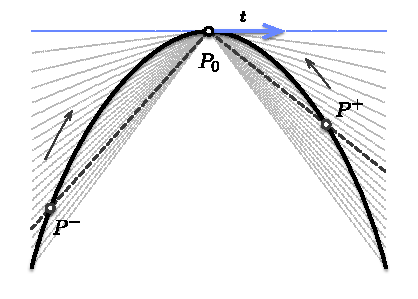
\includegraphics{frenet_tangent.pdf}\label{<figure1>}}
     \subfloat[][Curve's normal and osculating circle.]{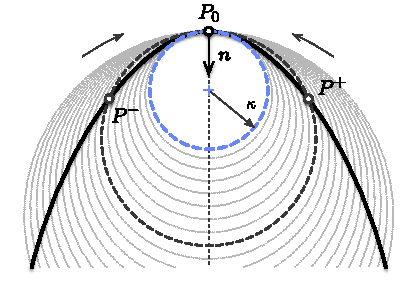
\includegraphics{frenet_normal.pdf}\label{<figure2>}}
     \caption{Differential definition of Frenet's trihedron at given point $P_0$.}
     \label{fig:3_1}
\end{figure}

%Normal vector
\subsection{Normal vector}
The second component of the Frenet trihedron is called the \emph{unit normal vector}. It is constructed from $\vect{t'}$ which is necessarily orthogonal to $\vect{t}$. Indeed :
\begin{equation}
	\norm{\vect{t}}=1 \Rightarrow \vect{t^{'}} \cdot  \vect{t} = 0 \Leftrightarrow  \vect{t^{'}} \perp \vect{t}
\end{equation}
Let $\gamma = (I,F)$ be a biregular parametric curve.\footnote{Note that $\vect{n}$ exists if only $\gamma$ is biregular, that is $\vect{t}'$ never vanishes or, equivalently, $\gamma$ is never locally a straight line.} Let $t \in I$ be a parameter. The \emph{unit normal vector} is defined as :
\begin{equation}
	\vect{n}(t) = \frac{\vect{t}'(t)}{\norm{\vect{t}'(t)}} 
	= \frac{\gamma'(t) \times (\gamma''(t) \times \gamma'(t))}{\norm{\gamma'(t)}^3}
	\quad,\quad
	\norm{\vect{n}(t)}=1
\end{equation}
For a curve parametrized by arc length, this expression simply becomes :
\begin{equation}
	\vect{n}(s) = \frac{\vect{t}'(s)}{\norm{\vect{t}'(s)}} 
	= \gamma'(s) \times (\gamma''(s) \times \gamma'(s))
	\quad,\quad
	s \in [0,L]
\end{equation}
In differential geometry, the unit normal to the curve $\gamma$ at point $P_0$ is obtained as the limit of the (normalized) vector $\overrightarrow{P_0 P^+}-\overrightarrow{P_0 P^-}$, as $P^-$ and $P^+$ approche $P_0$ respectively from its left and right sides (\cref{fig:3_1}) :
\begin{equation}
	\vect{n}(P_0)
	= \lim_{}\frac{\overrightarrow{P_0 P^+}-\overrightarrow{P_0 P^-}}{\norm{\overrightarrow{P_0 P^+}-\overrightarrow{P_0 P^-}}}
\label{eq:3_4}
\end{equation}
Remark that the notion of \emph{normal vector} is ambiguous for non-planar curves as there is an infinite number of possible normal vectors lying in the plane orthogonal to the curve's tangent. In practice, the tangent derivative is a convenient choice as it allows to extend the notion of curvature from planar to non-planar space curves. However, we will see (\cref{sec:bishop}) that other kind of trihedron can be constructed regarding this choice and that one of them is especially suitable for the study of slender beams.

%Binormal vector and torsion
\subsection{Binormal vector}
The third vector of Frenet's trihedron is called the \emph{unit binormal vector}. It is constructed from $\vect{t}$ and $\vect{n}$ to form an orthonormal direct basis of $\mathbb{R}^{3}$. 
Let $\gamma = (I,F)$ be a biregular parametric curve. Let $t \in I$ be a parameter. The \emph{unit binormal vector} is defined as :
\begin{equation}
	\vect{b}(t) = \vect{t}(t) \times \vect{n}(t)
	= \frac{\gamma'(t) \times \gamma''(t)}{\norm{\gamma'(t) \times \gamma''(t)}}
	\quad,\quad
	\norm{\vect{b}(t)}=1
\end{equation}
For a curve parametrized by arc length, this expression simply becomes :
\begin{equation}
	\vect{b}(s) = \vect{t}(s) \times \vect{n}(s)
	= \gamma'(s) \times \gamma''(s)
	\quad,\quad
	s \in [0,L]
\end{equation}

% Osculating plane
\subsection{Osculating plane}\label{sec:osculatingplane}
The tangent and normal unit vectors $\{\vect{t},\vect{n}\}$ form an orthonormal basis of the so-called \emph{osculating plane}, whereas the binormal vector $(\vect{b})$ is orthogonal to it. This plane is of prime importance because it is the plane in which the curve takes its curvature (see \cref{sec:curvature}).

As reported in \cite[p.45]{Delcourt2007}, the osculating plane seems to have been first introduced by Bernoulli as the plane passing through three infinitely near points on a curve.\footnote{\blockcquote[p.113]{Bernoulli1728}{Voco autem planum osculans, quod transit per tria curvae quaesitae puncta infinite sibi invicem propinqua}.
} Likewise, in modern differential geometry, the osculating plane is defined as the limit of the plane passing through the points $P^-$, $P_0$ and $P^+$ while $P^-$ and $P^+$ approche $P_0$ respectively from its left and right side (\cref{fig:3_1}).

Note that the normal unit vector and the binormal unit vector $\{\vect{n},\vect{b}\}$ define the so-called \emph{normal plane}, while the normal tangent vector and the binormal unit vector $\{\vect{t},\vect{b}\}$ define the so-called \emph{rectifying plane}. This planes are secondary for the present study.

% --------------------------------------------------------------------------------------------------------------------------------------------
% CURVE INVARIANTS
% --------------------------------------------------------------------------------------------------------------------------------------------

\section{Curves of double curvature}

The study of space curves belongs to the field of differential geometry. According to \cite[p.28]{Delcourt2007}, the terminology \emph{curve of double curvature} is attributed to Pitot around 1724.\footnote{\blockcquote[p.28]{Pitot1726}{Les Anciens ont nommé cette courbe Spirale ou Hélice ; parce que la formation sur le cylindre suit la même analogie que la formation d’une spirale ordinaire sur un plan; mais elle est bien différente de la spirale ordinaire, étant une des courbes à double courbure, ou une des lignes qu’on conçoit tracée sur la surface des Solides. Peut-être que ces sortes de courbes à double courbure, ou prises sur la surface des Solides, feront un jour l’objet des recherches des géomètres. Celle que nous venons d’examiner est, je crois, la plus simple de toutes.
}} However, as stated in \cite[p.321]{Coolidge2013} curvature and torsion where probably first thought by Monge around 1771.\footnote{\blockcquote[p.363]{Monge1809}{On appelle point d'inflexion, dans une courbe plane, le point où cette ligne, après avoir été concave dans un sens, cesse de l'être pour devenir concave dans l'autre sens. Il est évident que dans ce point, la courbe perd sa courbure, et que les deux élémens consécutifs sont en ligne droite. Mais une courbe à double courbure peut perdre chacune de ses courbures en particulier, ou les perdre toutes deux dans le même point ; c'est-à-dire, qu'il peut arriver ou que trois élémens consécutifs d'une même courbe à double courbure se trouvent dans un même plan, ou que deux de ces élémens soient en ligne droite. Il suit de là que les courbes à double courbure peuvent avoir deux espèces d'inflexions; la première a lieu lorsque la courbe devient plane, et nous l'appellerons simple inflexion; la seconde, que nous appellerons double inflexion, a lieu lorsque la courbe devient droite dans un de ses points.}.} It is also interesting to note that, at that time, \textquote{curvature} was also referred to as \textquote{flexure}, reflecting that the study of physical problems (e.g.\ \emph{elastica}) and the study of curves of double curvature were intimately related to each other.

Space curves were historically understood as \emph{curves of double curvature} by extension to the case of planar curves, where the curvature measures the deviance of a curve from being a straight line. The second curvature, nowadays known as the \textquote{torsion} or \textquote{second generalized curvature}, measures the deviance of a curve from being plane. 

%\note{arclength is a Euclidean invariant of the curve.}

\begin{figure}[t]
	\centering
	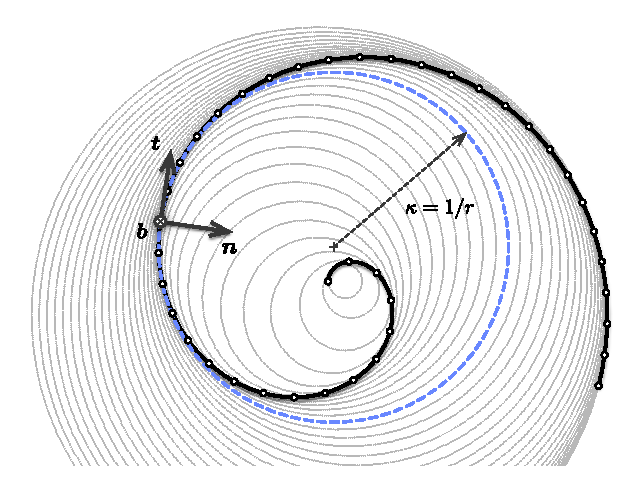
\includegraphics[]{osculating_circle.pdf}
	\caption{Osculating circles for a spiral curve at different parameters.}
	\label{fig:3_2}
\end{figure}

%Curvature
\subsection{First invariant : the curvature}\label{sec:curvature}
In differential geometry, the \emph{osculating circle} is defined as the limit of the circle passing through the points $P^-$, $P_0$ and $P^+$ while $P^-$ and $P^+$ approche $P_0$ (\cref{fig:3_1}). This circle lies on the osculating plane and its radius is nothing but the inverse of the local curvature of a curve.\footnote{ As explained by Euler itself, at a given arc length parameter ($s$), the osculating plane is the plane in which a curve takes its curvature : \blockcquote[p.364]{Euler1775}{in quo bina fili elementa proxima in curvantur}.} While the tangent gives the best local approximation of the curve as a straight line, the osculating circle gives the best local approximation of that curve as an arc.

The curvature is also known to be the \emph{gradient of arc length} (see \cite[p.4]{Vouga2014}) and calculated as : $\nabla{L} = \kappa \vect{n}$. Thus, the curvature gives the first-order variation in arc length when deforming a curve $\gamma$ in a closed enough curve $\gamma + \epsilon \delta\gamma$ :
\begin{equation}
	L(\gamma + \epsilon \delta\gamma) = L(\gamma) + \epsilon (\nabla L \cdot \delta\gamma) + o(\epsilon)
	\quad , \quad
	\nabla L \cdot \delta\gamma
	= \frac{d}{d\epsilon}L(\gamma+\epsilon \delta \gamma)\Bigr|_{\epsilon = 0}
%	= \lim_{\epsilon \to 0} \frac{L(\gamma+\epsilon \delta \gamma) - L(\gamma)}{\epsilon} 
%	=  \scalar{\nabla L}{\delta\gamma}
%	\quad , \quad
%	\nabla L = \scalar{\kappa \vect{n}}{\delta\gamma}
\end{equation}
This is easily understood in the case of a circle of radius $r$ extended to a circle of radius $r+dr$, where the total arc length variation is given by : 
$L(r + dr) - L(r) = \kappa dr L(r) $.

Note that due to the inner product with the normal vector, only the normal component of the deformation results in an effective extension of the curve. This point is worth to note as it will be related to the \emph{inextensibility assumption} made later in our beam model.

\subsubsection{Curvature}
Let $\gamma$ be a regular arc length parametrized curve. Let $s \in [0,L]$ be an arc length parameter. The \emph{curvature} is a positive scalar quantity defined as :
\begin{equation}
	\kappa(s) = \norm{\vect{t}'(s)} \ge 0 
	\quad,\quad
	\vect{t}'(s) = \kappa(s) \vect{n}(s)
\label{eq:curvaturedef}
\end{equation}
The curvature is \emph{independent} regarding the choice of parametrization. This makes the curvature an \emph{intrinsic property} of a given curve and that is why it is also referred to as a \emph{geometric invariant}. Following \cite[pp.203-204]{Gray2006} it can be computed for any parametrization $(I,F)$ of $\gamma$ as :
\begin{equation}
	\kappa(t) = \frac{\norm{\gamma'(t) \times \gamma''(t)}}{\norm{\gamma'(t)}^3}
	\quad,\quad
	\vect{t}'(t) = \norm{\gamma'(t)} \kappa(t) \vect{n}(t)
\label{eq:curvaturedef2}
\end{equation}
Note that in \cref{eq:curvaturedef} the prime denotes the derivative regarding the natural parameter ($s$) while it denotes the derivative regarding any parameter ($t$) in \cref{eq:curvaturedef2}. Consequently, the \emph{speed} of the curve's parametrization appears in the latter equation :
\begin{equation}
	v(t) = \frac{ds}{dt} = \norm{\gamma'(t)} = s'(t)
\end{equation}
The curvature measures how much a curve \emph{bends instantaneously} in its osculating plane, that is how fast the tangent vector is rotating in the osculating plane around the binormal vector. In differential geometry this is expressed as :
\begin{equation}
	\kappa(s)
	= \lim_{ds \to 0}\frac{\angle(\vect{t}(s),\vect{t}(s+ds))}{ds}
	= \lim_{ds \to 0}\frac{(\vect{t}(s+ds) - \vect{t}(s)) \cdot \vect{n}(s)}{ds}
\end{equation}
This is equivalent as measuring how fast the osculating plane itself is rotating around the binormal vector. Consequently a curve is locally a \emph{straight line} when its curvature vanishes ($\kappa(s)= 0$).

%Radius of curvature
\subsubsection{Radius of curvature}
The \emph{radius of curvature} is defined as the inverse of the curvature ($r= 1/\kappa$). From a geometric point of view, one can demonstrate that it is the radius of the osculating circle (\cref{fig:3_2}). Remark that where the curvature vanishes the radius of curvature goes to infinity ; that is the osculating circle becomes a line, a circle of infinite radius.

%Osculating circle
\subsubsection{Center of curvature}
The \emph{center of curvature} is defined as the center of the osculating circle (\cref{fig:3_2}). The locus of all the centers of curvature of a curve is called the \emph{evolute}.

\subsubsection{Curvature binormal vector}
\label{sec:kb}
Finally, following \cite{Bergou2008} we define the \emph{curvature binormal vector}. Let $\gamma$ be a biregular arc length parametrized curve. Let $s\in [0,L]$ be an arc length parameter. The \emph{curvature binormal vector} is defined as :
\begin{equation}
	\vect{\kappa b}(s) = \vect{t}(s) \times \vect{t}'(s) = \kappa(s)\cdot\vect{b}(s)
	\quad,\quad
	\norm{\vect{\kappa b}(s)}= \kappa(s)
\label{eq:kb}
\end{equation}
This vector will be useful as it embed all the necessary information on the curve's curvature. We will see (\cref{sec:bishopvelocity}) that this vector is associated to the angular velocity of a specific adapted moving frame attached to the curve and called the \emph{Bishop frame}.

% Torsion
\subsection{Second invariant : the torsion}\label{sec:torsion}
Let $\gamma$ be a biregular arc length parametrized curve. Let $s \in [0,L]$ be an arc length parameter. The \emph{torsion} is a scalar quantity defined as :
\begin{equation}
	\tau_f(s) = \vect{n}'(s) \cdot \vect{b}(s) = - \vect{b}'(s) \cdot \vect{n}(s)
\end{equation}
The torsion is \emph{independent} regarding the choice of parametrization. This makes the torsion an \emph{intrinsic property} of a given curve and that is why it is also referred to as a \emph{geometric invariant}. Following \cite[p.204]{Gray2006} it can be computed for any parametrization $(I,F)$ of $\gamma$ as :
\begin{equation}
	\tau_f(t) = \frac{(\gamma'(t) \times \gamma'(t)) \cdot \gamma''(t)}{\norm{\gamma'(t) \times \gamma''(t)}^2}
	\quad when \quad
	\kappa(t) > 0
\end{equation}
The torsion measures how much a curve goes \emph{instantaneously out of its plane}, that is to say how fast the normal or binormal vectors are rotating in the normal plane around the tangent vector. In differential geometry this is expressed as :
\begin{equation}
	\tau_f(s) 
	= \lim_{ds \to 0}\frac{\angle(\vect{n}(s),\vect{n}(s+ds))}{ds}
	= \lim_{ds \to 0}\frac{(\vect{n}(s+ds) - \vect{n}(s)) \cdot \vect{b}(s)}{ds}
\end{equation}
This is equivalent as measuring how fast the osculating plane is rotating around the tangent vector. Consequently a curve is locally \emph{plane} when its torsion vanishes ($\tau_f(s) = 0$).

Remark that the \emph{torsion} is denoted \textquote{$\tau_f$} and not simply \textquote{$\tau$} as the latter will be reserved to denote any angular velocity of a moving adapted frame around its tangent vector. Thus, $\tau_f$ refers to the particular angular velocity of the Frenet trihedron around it's tangent vector. This torsion, which is a geometric property of the curve, will be indifferently referred to as the \emph{Frenet torsion} or the \emph{geometric torsion}.

% Fundamental theorem of space curves
\subsection{Fundamental theorem of space curves}\label{sec:fundamental}
This two \emph{generalized curvatures}, respectively the curvature ($\kappa$) and the torsion ($\tau_f$), are \emph{invariant} regarding the choice of parametrization and under \emph{euclidean motions}. The \emph{Fundamental theorem of space curves} states that a curve is fully described, up to a Euclidean motion of ${\mathbb{R}}^3$, by its positive curvature ($\kappa > 0$) and torsion ($\tau$) \cite[p.229]{Gray2006}.

% The Serret-Frenet formulas
\subsection{Serret-Frenet formulas}\label{sec:serret}
The \emph{Fundamental theorem of space curves} is somehow a consequence of the \emph{Serret-Frenet formulas}, which is the first-order system of differential equations satisfied by the Frenet trihedron. Let $\gamma$ be a biregular arc length parametrized curve. Let $s \in [0,L]$ be an arc length parameter. Then, the Frenet trihedron satisfies the following formulas :
\begin{equation}
	\left\{
	\begin{aligned}
		&\vect{t^{'}}(s) 	=  \kappa_{}(s) \vect{n}(s)\\
		&\vect{n^{'}}(s) 	=  -\kappa_{}(s) \vect{t}(s) + \tau_f(s) \vect{b}(s) \\
		&\vect{b^{'}}(s) 	=  -\tau_f(s) \vect{n}(s) \\
	\end{aligned}
	\right.
\end{equation}
This system can be seen as the \emph{equations of motion} of the Frenet trihedron moving along the curve $\gamma$ at unit speed ($\norm{\gamma'}=1$). Indeed, introducing its \emph{angular velocity vector} also known as the \emph{Darboux vector} ($\vect{\Omega_f}$), the previous system is expressed as :
\begin{equation}
	\begin{bmatrix}		
		\vect{t^{'}}(s) \\
		\vect{n^{'}}(s) \\
		\vect{b^{'}}(s) \\
	\end{bmatrix}
	=
	\vect{\Omega_f}(s)
	\times
	\begin{bmatrix}		
		\vect{t}(s) \\
		\vect{n}(s) \\
		\vect{b}(s) \\
	\end{bmatrix}
	\quad where \quad
	\vect{\Omega_f}(s)
	=
	\begin{bmatrix}
		\tau_f(s) \\
		0 \\
		\kappa(s)
	\end{bmatrix}
\end{equation}
Because the Frenet trihedron satisfies a first-order system of differential equations of parameters $\kappa$ and $\tau_f$ it is possible, by integration, to reconstruct the trace of the moving frame and thus the curve, up to a constant of integration (a trihedron in this case).
%For instance, those classic combinations of curvature and torsion leads to :
%\begin{itemize}
%	\item a curve of null curvature and null torsion is a straight line ;
%	\item a curve of constant curvature and null torsion is a circle ;
%	\item a curve of constant curvature and constant torsion is a circular helix.
%\end{itemize}

Finally, those formulas can be generalized to any non unit-speed parametrization of a curve\footnote{See \cite[p.203]{Gray2006} for a complete proof.}. Let $\gamma = (I,F)$ be a biregular parametric curve. Let $t \in I$ be a parameter. Then the following \emph{generalized Serret-Frenet formulas} hold :
\begin{equation}
	\left\{
	\begin{aligned}
		&\vect{t^{'}}(t) 	=  v(t) \kappa_{}(t) \vect{n}(t)\\
		&\vect{n^{'}}(t) 	=  -v(t) \kappa_{}(t) \vect{t}(t) + v(t) \tau_f(s) \vect{b}(t) \\
		&\vect{b^{'}}(t) 	=  -v(t) \tau_f(t) \vect{n}(t) \\
	\end{aligned}
	\right.
\end{equation}
Again, this system can be seen as the \emph{equations of motion} of the Frenet trihedron moving along the curve $\gamma$ at non unit-speed ($v(t) = \norm{\gamma'(t)}$). This time the \emph{angular velocity vector} ($\vect{\Omega}$) is distinct from the \emph{Darboux vector} ($\vect{\Omega_f}$) and the previous system is expressed as :
\begin{equation}
	\begin{bmatrix}		
		\vect{t^{'}}(t) \\
		\vect{n^{'}}(t) \\
		\vect{b^{'}}(t) \\
	\end{bmatrix}
	=
	\vect{\Omega}(t)
	\times
	\begin{bmatrix}		
		\vect{t}(t) \\
		\vect{n}(t) \\
		\vect{b}(t) \\
	\end{bmatrix}
	\quad where \quad
	\vect{\Omega}(t)
	=
	v(t)
	\begin{bmatrix}
		\tau_f(t) \\
		0 \\
		\kappa(t)
	\end{bmatrix}
\end{equation}


\begin{figure}[t]
	\centering
	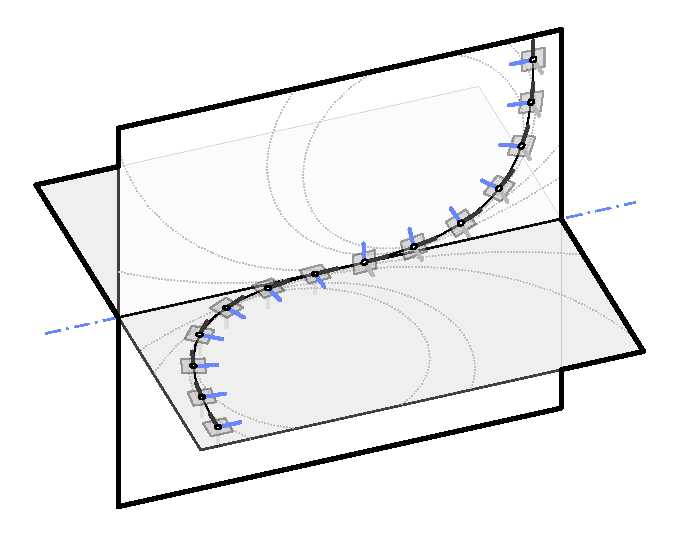
\includegraphics[]{frenet_torsion.pdf}
	\caption{Geometric torsion and rotation of the osculating plane. Note the existence of an inflexion point with a vanishing curvature and a discontinuity of both $\tau_f$ and the osculating plane.}
	\label{fig:3_3}
\end{figure}

% --------------------------------------------------------------------------------------------------------------------------------------------
% CURVE FRAMING
% --------------------------------------------------------------------------------------------------------------------------------------------

\section{Curve framing}

%From now on, we consider $\gamma$ to be a biregular arc length parametrized curve.

While the Frenet trihedron \blockcquote[p.1]{Bishop1975}{has long been the standard vehicle for analysing properties of the curve invariant\footnote{Namely the curvature ($\kappa$) and the Frenet torsion ($\tau_f$).} under euclidean motions}, a curve can be potentially framed with any arbitrary \emph{moving frame}, understood as an \emph{orthonormal basis field}. Thus, the Frenet frame is not the only way to frame a curve and other frames may or may not exhibit some interesting properties.\footnote{Recall the title of Bishop's paper : \blockcquote[]{Bishop1975}{There is more than one way to frame a curve}.} 

In his paper \cite{Bishop1975} Bishop establishes the differential equation that a moving frame must satisfy and remarks that, because of the orthnormality condition, the first derivatives of the frame components can be expressed in terms of themselves through a skew-symmetric coefficient matrix. For such a frame, the understanding of its motion along the curve is thus reduced to the knowledge of only three scalar coefficient functions. He remarks that most of the interesting properties that the Frenet frame exhibits are due to the fact that one of this coefficient function is vanishing everywhere on the curve (that is the frame is \emph{rotation-minimizing} regarding one of its components) ; and that the Frenet frame is \emph{adapted} to the curve (that is one of its components is nothing but the unit tangent vector).

In this section we introduce the \emph{moving frame} notion and two properties of interest such a frame can exhibit in addition, that is : to be \emph{adapted} to the curve ; and to be \emph{rotation-minimizing} regrading a given direction. We then reconsider the case of the Frenet frame regrading this mathematical framework. Finally, we introduce the \emph{zero-twisting} frame also known as the \emph{bishop} frame.\footnote{Named after Bishop who introduced it.} This tool will be fundamental for our futur study of slender beams.

% moving frame
\subsection{Moving frame}

Let $\gamma$ be a curve parametrized by arc length. A map $F$ which associates to each point of arc length parameter $s$ a direct orthonormal trihedron is said toi be a \emph{moving frame} :
\begin{equation}
	\fonctionL{F}{[0,L]}{\mathcal{SO}_{3}(\mathbb{R})}{s}{F(s) = \{\vect{e}_{3}(s),\vect{e}_{1}(s),\vect{e}_{2}(s)\}}
\end{equation}
Consequently, a moving frame $F$ attached to $\gamma$ satisfies for all $s \in [0,L]$ :
\begin{equation}
	\left\{
	\begin{aligned}
		& \norm{\vect{e}_i(s)} = 1 \\
		& \vect{e}_i(s) \cdot \vect{e}_j(s) = 0\quad , \quad i \neq j
	\end{aligned}
	\right.
\end{equation}
The term \textquote{moving frame} will refer indifferently to the map itself (denoted $F=\{\vect{e}_{3},\vect{e}_{1},\vect{e}_{2}\}$), or to a specific evaluation of the map (denoted $F(s)=\{\vect{e}_{3}(s),\vect{e}_{1}(s),\vect{e}_{2}(s)\}$).

% governing equations
\subsubsection{Governing equations}
Computing the derivatives of the previous relationships leads to the following system of differential equations that the frame must satisfy for all $s \in [0,L]$ :
\begin{equation}
	\left\{
	\begin{aligned}
		&\vect{e}'_i(s) \cdot \vect{e}_i(s) = 0 \\
		&\vect{e}'_{i}(s) \cdot \vect{e}_{j}(s) = -\vect{e}_{i}(s) \cdot \vect{e}'_{j}(s)\quad , \quad i \neq j
	\end{aligned}
	\right.
\end{equation}
Thus, there exists 3 scalar functions ($\tau$, $k_{1}$, $k_{2}$) such that $\{\vect{e}'_{3}, \vect{e}'_{1}, \vect{e}'_{2}\}$ can be expressed in the basis $\{\vect{e}_{3}, \vect{e}_{1}, \vect{e}_{2}\}$ :
\begin{equation}
	\left\{
	\begin{aligned}
		&\vect{e}'_{3}(s) = k_{2}(s)\vect{e}_{1}(s) - k_{1}(s)\vect{e}_{2}(s) \\
		&\vect{e}'_{1}(s) = -k_{2}(s)\vect{e}_{3}(s) + \tau(s)\vect{e}_{2}(s) \\
		&\vect{e}'_{2}(s) = k_{1}(s)\vect{e}_{3}(s) - \tau(s)\vect{e}_{1}(s)
	\end{aligned}
	\right.
\end{equation}
It is common to rewrite this first-order linear system of differential equations as a matrix equation : \footnote{In the case of a space curve, where $\vect{e}_3$ is chosen to be the curve tangent unit vector and $\vect{e}_1$ is chosen to be the curve normal unit vector, this set of equations is known as the \emph{Serret-Frenet formulas}.}\textsuperscript{,}\footnote{In the case of a space curve drawn on a surface, where $\vect{e}_3$ is chosen to be the curve tangent unit vector and $\vect{e}_1$ is chosen to be the surface normal unit vector, this set of equations is known as the \emph{Darboux-Ribaucour formulas}.}
\begin{equation}
	\begin{bmatrix}
		\vect{e}'_{3}(s) \\
		\vect{e}'_{1}(s) \\
		\vect{e}'_{2}(s)
	\end{bmatrix}
	=
	\begin{bmatrix}
		0 & k_{2}(s) & -k_{1}(s) \\
		-k_{2}(s) & 0 & \tau(s) \\
		k_{1}(s) & -\tau(s) & 0
	\end{bmatrix}
	\begin{bmatrix}
		\vect{e}_{3}(s) \\
		\vect{e}_{1}(s) \\
		\vect{e}_{2}(s)
	\end{bmatrix}
\label{eq:movingframe}
\end{equation}
Since the progression of any moving frame along $\gamma$ is ruled by a first-order system of differential equations, a unique triplet $\{\tau, k_{1}, k_{2}\}$ leads to a set of moving frames equal to each other within a constant of integration.\footnote{This assumption reminds the \emph{Fundamental theorem of space curves} (\cref{sec:fundamental}).} Basically, with a given triplet $\{\tau, k_{1}, k_{2}\}$, one can propagate a given initial direct orthonormal trihedron (at $s=0$ for instance) through the whole curve by integrating the system of differential equations. In general, a moving frame will be fully determined by $\tau$, $k_{1}$ and $k_{2}$ together with the initial condition $\{\vect{e}_{3}(s=0),\vect{e}_{1}(s=0),\vect{e}_{2}(s=0)\}$.

\begin{figure}[t]
\centering
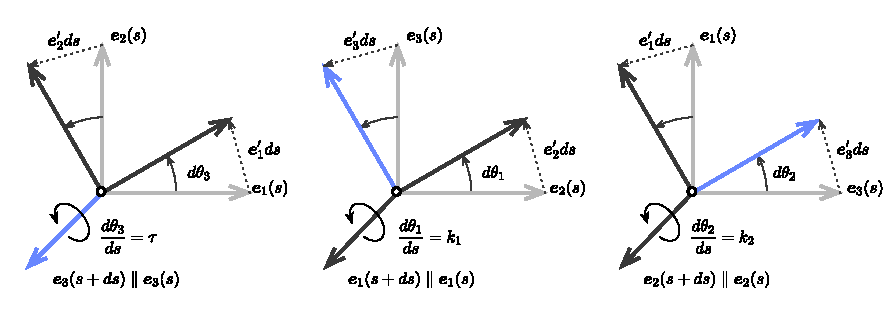
\includegraphics[]{darboux.pdf}
\caption{Geometric interpretation of the angular velocity vector of a moving frame.}
\label{fig:3_4}
\end{figure}

% ANGULAR VELOCITY VECTOR
\subsubsection{Angular velocity}
This system can be seen as the \emph{equations of motion} of the frame moving along the curve $\gamma$ at unit speed ($\norm{\gamma'}=1$). Indeed, introducing its \emph{angular velocity vector} ($\vect{\Omega}$), the previous system is expressed as :
\begin{equation}
	\vect{e}'_{i}(s) = \vect{\Omega}(s) \times \vect{e}_{i}(s)
	\quad avec \quad
	\vect{\Omega}(s)
	=
	\begin{bmatrix}
		\tau(s) \\
		k_1(s) \\
		k_2(s)
	\end{bmatrix}
\end{equation}
This result is straightforward deduced from \cref{eq:movingframe}. Note that the cross product reveals the skew-symmetric nature of the system, which could already be seen in \cref{eq:movingframe}.
Geometrically, decomposing the infinitesimal rotation of the moving frame around its directors between arc length $s$ and $s+ds$ (\cref{fig:3_4}) shows that the scalar functions $\tau$, $k_{1}$ and $k_{2}$ effectively correspond to the angular speed of the frame moving along $\gamma$, respectively around $\vect{e}_{3}$, $\vect{e}_{1}$ and $\vect{e}_{2}$ :
\begin{equation}
	\frac{d\theta_3}{ds}(s) = \tau(s)
	\quad,\quad
	\frac{d\theta_1}{ds}(s) = k_{1}(s)
	\quad,\quad
	\frac{d\theta_2}{ds}(s) = k_{2}(s)
\end{equation}

\begin{figure}[t]
\centering
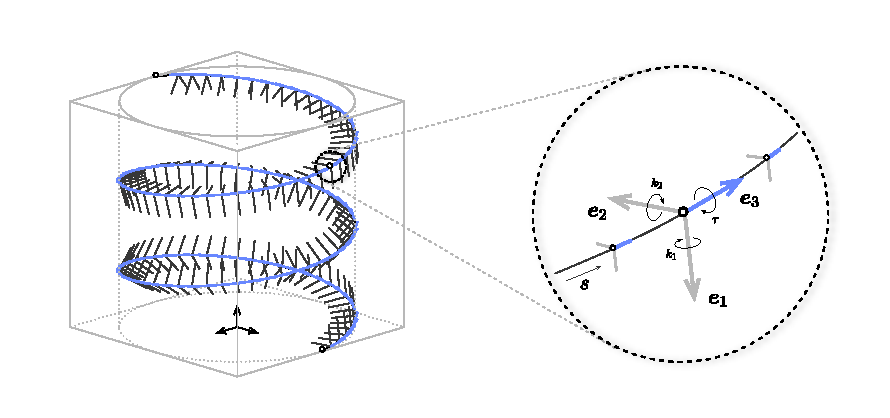
\includegraphics[]{adapted_moving_frame.pdf}
\caption{Adapted moving frame $F(s) =\{\vect{e}_{3}(s),\vect{e}_{1}(s),\vect{e}_{2}(s)\}$ where $\vect{e}_3(s) = \vect{t}(s)$.}
\label{fig:adapted}
\end{figure}

% ADAPTED FRAME
\subsection{Adapted moving frame}
\label{sec:amf}
Let $F$ be a moving frame as defined in the previous section. $F$ is said to be \emph{adapted} to $\gamma$ if at each point $\gamma(s)$, $\vect{e}_{3}(s)$ is the unit tangent vector of $\gamma$ (\cref{fig:adapted}) :
\begin{equation}
	\vect{e_{3}}(s) = \vect{t}(s) = \frac{\gamma^{'}(s)}{\norm{\gamma^{'}(s)}}
\end{equation}
For an adapted frame, the components $k_1$ and $k_2$ of the angular velocity vector are related to the curvature of $\gamma$\footnote{\note{Faire le lien avec l'énergie de flexion, qui ne dépend donc que de la géométrie de la courbe dans le cas d'une isotropic rod $\mathcal{E}_b = EI\kappa^2$.}} : 
\begin{equation}
	\kappa(s) = \norm{\vect{e}'_{3}(s)} = \norm{k_2(s)\vect{e}_1(s) + k_1(s)\vect{e}_2(s)} = \sqrt{{k_{1}(s)}^2 + {k_{2}(s)}^2}
\end{equation}
Moreover, recalling the definition of the curvature binormal vector ($\vect{\kappa b}$) from \cref{eq:kb}, it is easy to see that for an adapted moving frame the following relation holds :
 \begin{equation}
	\vect{\kappa b}(s) = k_1(s) \vect{e}_1(s) +  k_2(s) \vect{e}_2(s) \label{eq:amf_kb}
\end{equation}
Consequently, the angular velocity vector of an adapted moving frame can be written as :
 \begin{equation}
	\vect{\Omega}(s) = \vect{\kappa b}(s)  + \tau(s) \vect{t}(s)
\end{equation}
This last result is very interesting as it shows that any adapted moving frame will differ from each other only by their twisting speed as $\vect{\Omega}_{\perp} =  \vect{\kappa b}$ only depends on the curve.

% ROTATION MINIMIZING FRAME
\subsection{Rotation-minimizing frame}
Following \cite{Farouki2014, Wang2008} we introduce the \emph{rotation-miniminzing frame} notion. A frame $\{\vect{e}_{3}$, $\vect{e}_{1}$, $\vect{e}_{2}\}$ is said to be \emph{rotation-miniminzing} regrading a given direction $\vect{d}$ if :
\begin{equation}
	\vect{\Omega}(s) \cdot \vect{d}(s) = 0
\end{equation}

% PARALLEL TRANSPORT
\subsection{Parallel transport}\label{sec:paralleltransport}
The notion of \emph{parallel transport} is somehow a generalization of the classical notion of collinearity in flat euclidean spaces (e.g.\ $\mathbb{R}^2$ or $\mathbb{R}^3$), to spaces that exhibit some non vanishing curvature (e.g.\ spheric or hyperbolic spaces).\footnote{\url{https://www.youtube.com/watch?v=p1tfZD2Bm0w}}

\subsubsection{Relatively parallel fields}
Following \cite{Bishop1975}, we define what is a \emph{(relatively) parallel field}. Let $\gamma$ be a regular curve parametrized by arc length. Let $\vect{p}$ be a vector field along $\gamma$. The vector field $\vect{p}$ is said to be \emph{parallel} if its derivative is purely tangential, that is :
\begin{equation}
	\vect{p}'(s) \times \vect{t}(s) = 0
\end{equation}
Consequently, for an adapted moving frame, the \emph{normal fields} $\vect{e}_1$ and $\vect{e}_2$ are both \emph{relatively parallels} if and only if the frame angular velocity is itself a normal field, that is : \footnote{A vector field $\vect{p}$ is said to be \emph{normal} along a curve $\gamma$ if : $\forall s \in [0,L]$, $\vect{p}\cdot\vect{t} = 0$.}
\begin{equation}
	\vect{\Omega}(s) = \vect{\Omega}_{\perp}(s) =  \vect{\kappa b}(s) \Leftrightarrow \vect{\Omega}(s) \cdot \vect{t}(s) = 0  \Leftrightarrow \tau(s) = 0  
\end{equation}
In other words, a \emph{relatively parallel normal field} : \blockcquote{Bishop1975}{turns, only whatever amount is necessary for it to remain normal, so it is as close to being parallel as possible without losing normality}. 
%
%In addition, relatively parallel normal vector fields exhibit some interesting properties \cite{Hanson95} : 
%\begin{itemize}
%	\item $\|\vect{p}\|$ is of constant length;
%	\item $\|\vect{p}\|$ is of constant length;
%\end{itemize}

\subsubsection{Parallel transport of vectors along a curve}
Reciprocally, it is possible to define the \emph{parallel transport} of a vector along a curve $\gamma$ as its propagation along $\gamma$ at angular speed $\vect{\kappa b}$. An initial vector $\vect{p}_0 = \vect{p}(s_0)$ is parallel transported at arc length parameter $s$ into the vector $\vect{p}(s)$ by integrating the following first-order differential equation along $\gamma$ :
\begin{equation}
	\vect{p}'(s) = \vect{\kappa b}(s) \times  \vect{p}(s)
\end{equation}
Consequently, the resulting vector field $\vect{p}$ is a parallel field. Note that a parallel field is not necessarily a normal field. 

From the point of view of differential geometry, this means that the next vector $\vect{p}(s+ds)$ is obtained by rotating the previous one $\vect{p}(s)$ around the curve binormal $\vect{b}(s)$ by an infinitesimal angle $d\theta(s) = \kappa(s) ds$. Note that $\vect{b}(s)$ has the same direction as $\vect{t}(s) \times \vect{t}(s+ds)$.

\subsubsection{Parallel transport of frames along a curve}
Identically, the \emph{parallel transport} of an adapted frame is defined as the parallel transport of its components along $\gamma$.

%\subsubsection{Parallel curves and inextensibility}
%Let $\vect{p}$ be a \emph{relatively parallel normal vector field}.
%
%Relatively parallel fields \cite[p.4]{Carroll2007}, \cite{Bishop1975}, \cite{Hanson95}

% FRENET FRAME
\subsection{Frenet frame}
\label{sec:ff}

The Frenet frame is a well-known particular adapted moving frame. It is defined as the map that attach to any given point of $\gamma$ the corresponding Frenet trihedron $\{\vect{t}(s),\vect{n}(s),\vect{b}(s)\}$ where :
\begin{gather}
\vect{t}(s) = \frac{\gamma^{'}(s)}{\norm{\gamma'(s)}}
\quad,\quad
\vect{n}(s) = \frac{\vect{t'}(s)}{\kappa(s)}
\quad,\quad
\vect{b}(s)= \vect{t}(s)\times\vect{n}(s)
\end{gather}

\subsubsection{Governing equations}\label{sec:serretfrenet}
The Frenet frame satisfies the \emph{Frenet-Serret formulas} (see \cref{sec:serret}), which govern the evolution of the frame along the curve $\gamma$ :
\begin{equation}
	\begin{bmatrix}
		\vect{t^{'}}(s) \\
		\vect{n^{'}}(s) \\
		\vect{b^{'}}(s)
	\end{bmatrix}
	=
	\begin{bmatrix}
		0 & \kappa_{}(s) & 0 \\
		-\kappa_{}(s) & 0 & \tau_f(s) \\
		0 & -\tau_f(s) & 0
	\end{bmatrix}
	\begin{bmatrix}
		\vect{t}(s) \\
		\vect{n}(s) \\
		\vect{b}(s)
	\end{bmatrix}
\label{eq:frenetframegoverning}
\end{equation}
Remember the generic system of differential equations of an adapted moving frame attached to a curve, established in \cref{eq:movingframe}, where :
\begin{gather}
\vect{e_{3}}(s) = \vect{t}(s)
\quad,\quad
k_{1}(s) = 0
\quad,\quad
k_{2}(s) = \kappa(s)
\quad,\quad
\tau(s) = \tau_{f}(s)
\end{gather}

\subsubsection{Angular velocity}
Consequently, the angular velocity vector ($\vect{\Omega_{f}}$) of the Frenet frame, also known as the \emph{Darboux vector} in this particular case, is given by :
\begin{equation}
	\vect{\Omega_f}(s)
	=
	\begin{bmatrix}
		\tau_{f}(s) \\
		0 \\
		\kappa(s)
	\end{bmatrix}
	= \vect{\kappa b}(s) +\tau_{f}(s) \vect{t}(s)
\end{equation}
Remark that the Frenet frame satisfies $\vect{\Omega_f}(s) \cdot \vect{n}(s) = 0$ and is thus a \emph{rotation-miniminzing} frame regarding the normal vector ($\vect{n}$). The motion of this frame through the curve is known as \textquote{pitch-free}.

Note also that $\vect{t^{'}}(s)$ and $\vect{b^{'}}(s)$ are colinear to $\vect{n}(s)$. This means that the projection of $\vect{t}(s)$ and $\vect{b}(s)$ is conserved from one normal plane to another, that is $\vect{t}$ and $\vect{b}$ are parallel transported along the vector field $\vect{n}$.

\subsubsection{Drawbacks and benefits}\label{sec:frenetdrawbacks}
\footnote{\note{une perturbation de la courbe dans le sens de la courbure engendre une variation de longueur de la courbe proportionnelle à l'inverse de la courbure (au premier ordre) + schéma.}}\textsuperscript{,}\footnote{\note{une perturbation de la courbe dans le sens de la binormale (en tout point) préserve la longueur de la courbe au 1er ordre : c'est un déplacement qui conserve l'hypothèse d'inextensibilité au premier ordre.}}\textsuperscript{,}\footnote{\note{Examiner la question de la fermeture sur une boucle fermée. Schéma.}}

The Frenet frame is not continuously defined if $\gamma$ is not $\mathcal{C}^2$. This is problematic for the study of slender beams as the centerline of a beam subject to punctual external forces and moments or to material discontinuities will not be $\mathcal{C}^2$ but only picewise $\mathcal{C}^2$. In that case, the centerline tangent will be continuously defined everywhere but the curvature will be subject to discontinuities, that is $\vect{t}'$ will not be continuously defined.

Moreover, even if $\gamma$ is $\mathcal{C}^2$, the Frenet frame is not defined where the curvature vanishes, which obviously is an admissible configuration for a beam centerline. This issue can be partially addressed by parallel transporting the normal vector along the straight regions of the curve. Thus, the extended frame will still satisfy the governing equations exposed in \cref{eq:frenetframegoverning}. However, if the osculating planes are not parallels on both sides of a region of null curvature, torsion will be subject to a discontinuity and so the Frenet frame (\cref{fig:3_3}).\footnote{This is also highlighted in \cite{Bloomenthal1990, Wang2008}.} Again, if the region of null curvature is not a point, that is the region is not an inflexion point but a locus where the curve is locally a straight line, the change in torsion on both sides of the region can be accommodated by a continuous rotation from one end to the other.

One benefit of the Frenet frame is that, when transported along a \emph{closed curve}, the frame at the end of the curve will align back with the frame at the beginning of the curve, that is the frame will returns to its initial value after a complete turn. During its trip, the frame will make a total twist of $\int_0^L \tau_f(s)ds = 0[2\pi]$ around the tangent vector.

A second benefit is that any adapted frame can be obtained by a rotation of the Frenet frame around the unit tangent vector \cite[p.2]{Guggenheimer1989}.

% BISHOP FRAME
\subsection{Bishop frame}\label{sec:bishop}

A \emph{Bishop frame} denoted $\{\vect{t},\vect{u},\vect{v}\}$, also known as \emph{zero-twisting} or \emph{parallel-transported} frame, is an adapted moving frame that has no tangential angular velocity : \footnote{Bishop frames were Introduced as \emph{relatively parallel adapted frames} in \cite{Bishop1975}.}
\begin{equation}
	\vect{\Omega} \cdot \vect{t} = \tau =\vect{u^{'}} \cdot \vect{v} = - \vect{u} \cdot \vect{v^{'}} = 0
\end{equation}
Because a Bishop frame is an adapted frame, it can be defined relatively to the Frenet frame by a rotation around the unit tangent vector. A Bishop frame is a frame that cancels out the rotational movement of the Frenet frame around the tangent vector. At arc length parameter $s$, the Frenet frame has continuously rotated around its tangent vector of a cumulative angle : $\int_0^s \tau_f(t)dt$. Thus, any Bishop frame will be obtained, within a constant rotation angle $\theta_0$, through a rotation of the Frenet frame around the tangent vector by an angle :
\begin{equation}
	\theta(s)  =  - \int_0^s \tau_f(t)dt + \theta_0(s)
\end{equation}
Consequently, a Bishop frame can be expressed relatively to the Frenet frame as :
\begin{equation}
	\left\{
	\begin{aligned}
		&\vect{u} = \cos \theta \vect{n} +  \sin \theta \vect{b}\\
		&\vect{v} = -\sin \theta \vect{n} +  \cos \theta \vect{b}
	\end{aligned}
	\right.
\end{equation}
\subsubsection{Governing equations}
The Bishop frame satisfies the following system of differential equations, which govern the evolution of the frame along the curve $\gamma$ :
\begin{equation}
	\begin{bmatrix}
		\vect{t^{'}}(s) \\
		\vect{u^{'}}(s) \\
		\vect{v^{'}}(s)
	\end{bmatrix}
	=
	\begin{bmatrix}
		0 & \kappa(s) \sin \theta(s) & -\kappa(s) \cos \theta(s) \\
		-\kappa(s) \sin \theta(s) & 0 & 0 \\
		\kappa(s) \cos \theta(s) & 0 & 0
	\end{bmatrix}
	\begin{bmatrix}
		\vect{t}(s) \\
		\vect{u}(s) \\
		\vect{v}(s)
	\end{bmatrix}
\label{eq:3_12}
\end{equation}
One can remember the generic differential equations of an adapted moving frame attached to a curve, where : \footnote{
\begin{equation*}
	\begin{aligned}
		&\tau =\vect{u^{'}} \cdot \vect{v} = (\vect{\Omega_f} \times \vect{u} + \theta^{'} \vect{v})\cdot  \vect{v} = \tau_f - \tau_f = 0\\
		&k_1 = -\vect{t^{'}} \cdot \vect{v} = -\kappa \vect{n} \cdot \vect{v} = \kappa \sin \theta \\
		&k_2 = \vect{t^{'}} \cdot \vect{u} = \kappa \vect{n} \cdot \vect{u} = \kappa \cos \theta
	\end{aligned}
\end{equation*}
}
\begin{equation}
k_{1}(s) = \kappa(s) \sin \theta(s)
\quad,\quad
k_{2}(s) = \kappa(s) \cos \theta(s)
\quad,\quad
\tau(s) = 0
\end{equation}

\subsubsection{Angular velocity}\label{sec:bishopvelocity}
Consequently, the angular velocity vector ($\vect{\Omega_{b}}$) of the Bishop frame is given by :
\begin{equation}
	\vect{\Omega_b}(s) 
	=
	\begin{bmatrix}
		0\\
		\kappa(s) \sin \theta(s)\\
		\kappa(s) \cos \theta(s)
	\end{bmatrix}
	= \vect{\kappa b}(s) 
\end{equation}
Remark that the Bishop frame satisfies $\vect{\Omega_b}(s) \cdot \vect{t}(s) = 0$ and is thus \emph{rotation-miniminzing} regarding the tangent vector. The motion of this frame through the curve is known as \textquote{roll-free}.

Because the motion of this frame is described by an angular velocity vector that is nothing but the curvature binormal vector ($\vect{\Omega_b} = \vect{\kappa b}$), it can be interpreted in terms of \emph{parallel transport} as defined in \cref{sec:paralleltransport}. Thus, given an initial frame at arc length parameter $s=0$, the Bishop frame at any arc length parameter ($s$) is obtained by parallel transporting the initial frame $\{\vect{t}(0),\vect{u}(0), \vect{v}(0)\}$ along the curve from $0$ to $s$.

\subsubsection{Drawbacks and benefits}
\footnote{\cite{Guggenheimer1989, Klok1986, Bloomenthal1990, Wang2008, Poston1995, Menninger2013}}\textsuperscript{,}\footnote{\blockcquote[p.6]{Wang2008}{Regarder la méthode de la bi-reflexion pour le calcul du repère de bishop}}

One of the main benefits of the Bishop frame is that its generative method : \blockcquote{Bloomenthal1990}{is immune to degeneracies in the curvature vector}. Although we first expressed the construction of the Bishop frame relatively to the Frenet frame (which exists wherever $\gamma$ is biregular), the existence of the Bishop frame, understood in terms of parallel transport, is guaranteed wherever the curvature binormal ($\vect{\kappa b} = \vect{t} \times \vect{t}'$) is defined. To be continuously defined over $[0,L]$, a Bishop frame only needs the curvature binormal vector to be picewise continuously defined over  $[0,L]$, which only requires that $\gamma'$ is $\mathcal{C}^0$ and that $\gamma''$ is picewise $\mathcal{C}^0$. Obviously, those weaker existence conditions are profitables to bypass the drawbacks of the Frenet frame regarding the modeling of slender beams listed in \cref{sec:frenetdrawbacks}.

Strictly speaking, a Bishop frame is not a reference frame as it is defined within an initial condition. However, we will see later that strains in a beam are modeled as a rate of change in the Bishop frame, and consequently the initial condition will disappear in the equations.

Unlike the Frenet frame, when transported along a \emph{closed curve}, the Bishop frame at the end of the curve will not necessarily align back with the frame at the beginning of the curve.\footnote{\blockcquote{Hanson95}{it is possible for closed curves to have parallel transport frames that do not match up after one full circuit of the curve}} Even if the frame returns to its initial value after a complete turn, it may returns in its position after several complete turns ($2k\pi$) around the curve tangent. During its trip, the frame will make a total twist of $\int_0^L \tau_f(s)ds = \alpha[2\pi]$ around the tangent vector. This difference of angle is related to the concept of  \emph{holonomy}.

Remark also that Frenet and Bishop frames coincide for planar curves ($\tau_f = 0$), within a constant rotation around the unit tangent vector.
 
 %related to mechanical torsion

%expliquer la notion de parallèle comme l'a formulé Laurent Hauswirth : la projection de $u'$ et $v'$ dans le plan normal à la tangente $t$ est nulle, cad que d'un plan à un autre la projection de $u$ et $v$ est conservée + faire schéma.

%Laurent Hauswirth : la complexité d'un problème est en général proportionnelle à la codimension de l'objet étudié et donc, de ce fait les courbes ($codim = 3-1 = 2$) sont des objets plus compliqués que les surfaces ($codim = 3-2=1$) ds $\mathbb{R}^3$.

\subsection{Comparison between Frenet and Bishop frames}

\subsubsection{Application A : circular helix}
Let $\gamma$ be a \emph{circular helix} of parameter $a$ and $k$. In a cartesian coordinate system, it is defined as :
\begin{equation}
	\vect{r}(t) 
	=
	\begin{bmatrix}
		a \cos t, a \sin t, k t
	\end{bmatrix}
	= a \cos t \, \vect{e}_x + a \sin t \, \vect{e}_y + k t \, \vect{e}_z
\end{equation}
The speed of this parametrization, the curvature and the geometric torsion are uniform and given by :
\begin{equation}
	v(t) = \sqrt{a^2+k^2}
	\quad,\quad
	\kappa(t) = \frac{a}{a^2 + k^2}
	\quad,\quad
	\tau_f(t) = \frac{k}{a^2 + k^2}
\end{equation}
The Frenet frame components are given by (with $\alpha = v \kappa$ and $\beta = v \tau_f$) :
\begin{equation}
	\begin{aligned}
	\vect{t}(t) &=
		\begin{bmatrix} 
			- \alpha \cos t, \alpha \sin t, \beta t 
		\end{bmatrix}
	\\
	\vect{n}(t) &= 
		\begin{bmatrix} 
			-\cos t, -\sin t, 0 
		\end{bmatrix}
	\\
	\vect{b}(t) &=
		\begin{bmatrix} 
			\beta \sin t, - \beta \cos t, \alpha
	\end{bmatrix} 	
	\end{aligned}
\end{equation}
And the Bishop frame components are given by :
\begin{equation}
	\begin{aligned}
		\vect{u}(t) &= 
		\begin{bmatrix} 	
			-\cos t \cos \beta t - \beta  \sin t \sin \beta t, -\sin t \cos \beta t + \beta  \cos t \sin \beta t, - \alpha \sin \beta t
		\end{bmatrix}
		\\
		\vect{v}(t) &= 
		\begin{bmatrix} 
			-\cos t \sin \beta t + \beta  \sin t \cos \beta t, -\sin t \sin \beta t - \beta  \cos t \cos \beta t, \alpha \cos \beta t
		\end{bmatrix}
	\end{aligned}
\end{equation}


soit pour une spirale dont on connait

\begin{figure}[H]
\centering
\subfloat[][Frenet frame]{%
  \begin{tikzpicture}
\begin{axis}[
	width = 7.5cm,
	xmin=-0.1, xmax= 1.1, restrict x to domain = 0 : 1,
	ymin=-4e-2, ymax= 7e-2, restrict y to domain = -4e-2:6e-2,
	ytick={-3e-2, 0, 3e-2, 6e-2},
	grid=major,
	]

 	\pgfplotstableread{ch3_geometry/plot/frenet_bishop_darboux/frenet.txt}\frenet;
	\addplot [Tblue, smooth, thick]
       	table [x expr=\thisrowno{0}, y expr=\thisrowno{2}] {\frenet};

	\pgfplotstableread{ch3_geometry/plot/frenet_bishop_darboux/frenet.txt}\frenet;
	\addplot [black, smooth, thick, dashed]
       	table [x expr=\thisrowno{0}, y expr=\thisrowno{3}] {\frenet};

	\pgfplotstableread{ch3_geometry/plot/frenet_bishop_darboux/frenet.txt}\frenet;
	\addplot [black, smooth, thick]
       	table [x expr=\thisrowno{0}, y expr=\thisrowno{4}] {\frenet};

\end{axis}
  \end{tikzpicture}}\quad
\subfloat[][Bishop frame]{%
  \begin{tikzpicture}
\begin{axis}[
	width = 7.5cm,
	xmin=-0.1, xmax= 1.1, restrict x to domain = 0 : 1,
	ymin=-4e-2, ymax= 7e-2, restrict y to domain = -4e-2:6e-2,
	ytick={-3e-2, 0, 3e-2, 6e-2},
	grid=major,
	]

       	\pgfplotstableread{ch3_geometry/plot/frenet_bishop_darboux/bishop.txt}\bishop;
	\addplot [Tblue, smooth, thick]
         table [x expr=\thisrowno{0}, y expr=\thisrowno{2}] {\bishop};

         \pgfplotstableread{ch3_geometry/plot/frenet_bishop_darboux/bishop.txt}\bishop;
	\addplot [black, smooth, thick, dashed]
         table [x expr=\thisrowno{0}, y expr=\thisrowno{3}] {\bishop};

         \pgfplotstableread{ch3_geometry/plot/frenet_bishop_darboux/bishop.txt}\bishop;
	\addplot [black, smooth, thick]
         table [x expr=\thisrowno{0}, y expr=\thisrowno{4}] {\bishop};


\end{axis}
  \end{tikzpicture}}
\caption[]{Comparison between Frenet and Bishop frame velocity for a spirale curve.}
\label{fig:3_6}
\end{figure}

% DISCRETE CURVES
% ================
\section{Discrete curves}

The previous section has introduced the fundamental analytical tools to develop a solid understanding of the geometry of smooth space curves. These tools will be essentials for the construction of the beam model presented later in \cref{sec:energy} and \cref{sec:krichhoff}. In this section, we look for equivalent notions in the case of discrete space curves, as the developed model will be implemented in a numerical program to solve real mechanical problems through a finite-difference method (see \cref{sec:discretization}).

The study of those discrete equivalent notions belong to the recent field of \emph{Discrete Differential Geometry} : \blockcquote[p.7]{Hoffmann2008}{In some sense discrete differential geometry can be considered more fundamental than differential geometry since the later can be obtained form the former as a limit}. In particular, we will see that they are several ways to define the discrete equivalents of the curvature and the unit tangent vector. Though these various ways are equivalent and match their smooth counterpart by passing to the limit, they exhibit different capabilities at the discrete level.

 \blockcquote[p.1]{Carroll2014}{There is no general theory or methodology in the literature, despite the ubiquitous use of discrete curves in mathematics and science. There are conflicting definitions of even basic concepts such as discrete curvature $\kappa$, discrete torsion $\tau$, or discrete Frenet frame.}.

%\cite{Hoffmann2008, Carroll2014, Crane2015, Vouga2014}

% definition
% ------------
\subsection{Definition}
\begin{figure}[t]
	\centering
	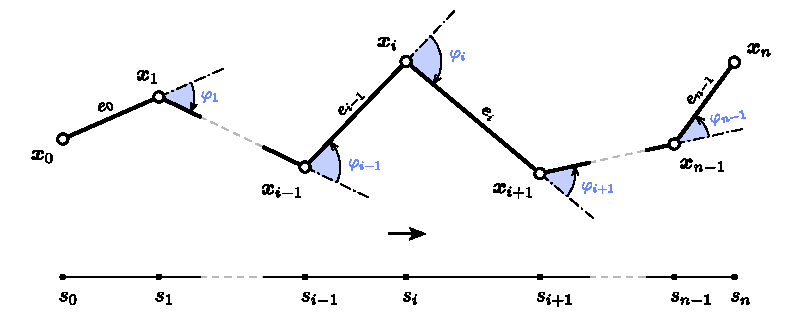
\includegraphics[]{discrete_curve_full.pdf}
	\caption{Discrete curve representation and parametrization.}
	\label{fig:discrete_curve}
\end{figure}

Let $\Gamma$ be a discrete (or polygonal) space curve. $\Gamma$ is defined as an ordered sequence $\Gamma = (\vect{x}_0,  \vect{x}_1, \ldots, \vect{x}_n) \in \mathbb{R}^{3(n+1)}$ of $n+1$ pairwise disjoint \emph{vertices} (see \cref{fig:discrete_curve}). Consecutive pairs of vertices define $n$ straight segments $(\vect{e}_0,  \vect{e}_1, \ldots, \vect{e}_{n-1})$ called \emph{edges}, pointing from one vertex to the next one : $\vect{e}_i = \vect{x}_{i+1} - \vect{x}_{i}$. The midpoint of $\vect{e}_i$ is a vertex denoted : $\vect{x}_{i+1/2} = \vect{x}_{i} + \frac{1}{2}\vect{e}_{i}$. The length of $\vect{e}_i$ is denoted $l_i = \norm{\vect{e}_i}$. The total length of $\Gamma$ is denoted $L = \sum_{i=0}^{n-1} \norm{\vect{e}_i}$. Additionally, we define the vertex-based mean length at vertex $\vect{x}_i$ : 
\begin{equation}
%\setlength{\jot}{8pt}
	\left\{
	\begin{alignedat}{4}
		\,	&\overbar{l_0} 		& = &\,	&& l_0					&\quad 	&i = 0		\\
			&\overbar{l_i}		& = &	&& \frac{1}{2}(l_{i-1} + l_i)		&		&i \in \llbracket 1, n-1 \rrbracket	\\
			&\overbar{l_n} 	\,	& = &	&& l_{n-1} 				&		&i = n		\\
	\end{alignedat}
	\right.
\end{equation}

\subsubsection{Discrete unit tangent vector}\label{sec:tangent_edge}
Edge vectors lead to a natural definition of the \emph{discrete unit tangent vector} along each edge : $\vect{u}_i = \vect{e}_i / l_i$. However, this definition makes no sens at vertices where all the curvature is \emph{condensed} and measured by the turning angle ($\varphi_i$). This is explained in terms of the Gau{\ss} map as edges will map to points but vertices will map to curves on the unit sphere.

\subsubsection{Discrete osculating plane}
Consecutive pairs of edges lead to a natural definition of the \emph{discrete osculating plane}, as the plane in which $\Gamma$ locally lies on. This plane is well defined by its normal vector known as the \emph{discrete unit binormal vector} ($\vect{b}_i = \frac{\vect{e}_{i-1} \times \vect{e}_{i}}{\norm{\vect{e}_{i-1} \times \vect{e}_{i}}}$) only if $\vect{e}_{i-1}$ and $\vect{e}_{i}$ are non-collinear ; that is the curve is not locally a straight line, or equivalently the curvature does not vanish.

\subsubsection{Discrete turning angle}
The \emph{turning angle} is defined as the oriented angle between to adjacent edges : $\varphi_i=\angle(\vect{e}_{i-1},\vect{e}_i)$. It is defined only for all $i \in \llbracket1,n-1\rrbracket$. It corresponds to the angle of rotation, in the osculating plane, around the binormal vector ($\vect{b}_i$), to align $\vect{e}_{i-1}$ with $\vect{e}_{i}$. The sign of $\varphi_i$ is taken in accordance to the right-hand rule regarding the orientation of $\vect{b}_i$. Thus, $\varphi_i$ is necessarily bounded to $[0,\pi]$ :
\begin{equation}
	0 \leqslant \varphi_i \leqslant \pi
\end{equation}
The next section will highlight the central role of the turning angle in the possible measurements of the discrete curvature.

Recall that for a planar curve, where $\varphi$ denotes the angle between the tangent vector ($\vect{t} = \cos\varphi \,\vect{e}_x + \sin\varphi \,\vect{e}_y$) and the horizontal line of direction $\vect{e}_x$, the following relation holds : $\varphi(s_1) - \varphi(s_2) = \int_{s_1}^{s_2} \frac{d \varphi}{d s} ds = \int_{s_1}^{s_2} \kappa ds$.

% parametrization
% ---------------------
\subsection{Regularity}

Let $\Gamma = (\vect{x}_0,  \vect{x}_1, \ldots, \vect{x}_n)$ be a discrete curve of edges $\vect{e}_0,  \vect{e}_1, \ldots, \vect{e}_{n-1}$. $\Gamma$ is said to be :
\begin{itemize}
	\item  \emph{regular} if it has no kinks : $\vect{e}_{i-1} + \vect{e}_{i} \neq 0 \Leftrightarrow \varphi_i \neq \pi \; | \; \forall i \in \llbracket 1,n-1 \rrbracket $
	\item  \emph{biregular} if no vertex is flat : $\vect{e}_{i-1} - \vect{e}_{i} \neq 0 \Leftrightarrow \varphi_i \neq 0 \; | \; \forall i \in \llbracket 1,n-1 \rrbracket $
\end{itemize}

% parametrization
% ---------------------
\subsection{Parametrization}

In the literature, discrete curves are usually considered as maps defined on $I = \llbracket 0,n \rrbracket \in \mathbb{N}^{n+1}$. As a consequence, the discrete derivative of $\Gamma$ is an edge-based quantity defined as : 
\begin{equation}
	\Gamma'_i = \frac{ \Gamma(t_{i+1}) -  \Gamma(t_i)}{t_{i+1} - t_i} = \vect{e}_i 
	\quad , \quad
	\vect{x}_{i} = \Gamma(t_i)
	\quad , \quad
	t_i = i
\end{equation}
Thus, as in the smooth case, a discrete curve is said to be parametrized by arc length if $\norm{\Gamma'} = 1$, that is every edges are of unit length ($\norm{\vect{e}_i} = 1$).\footnote{This assumption leads to the assertion that \blockcquote[p.10]{Hoffmann2008}{A discrete curve is parameterized by arc length or it is not}.} This constraint is sometimes relaxed to curves of constant edge length ($\norm{\vect{e}_i} = c$) that are said to be parametrized \emph{proportional} to arc length.

In the present work, to stick closer to the smooth case, we instead consider discrete curves as maps defined on $I = [t_0, t_1, \ldots, t_n] \in \mathbb{R}^{n+1}$ where $t$ denotes the discrete parametrization of $\Gamma$. As in the smooth case, the way to parametrized a curve is not unique.

\subsubsection{Arc length parameter}
By analogy with the smooth case, we define the curve arc length at vertices (see \cref{fig:discrete_curve}) as :
\begin{equation}
	\left\{
	\begin{aligned}
		s_0 	&= 0 								& 	&i = 0		\\
		s_i 	&= \sum_{k=1}^i \norm{\vect{e}_{k-1}}		&	&i \in \llbracket 1, n-1 \rrbracket	\\
		s_n 	&=  L 								&	&i = n		\\
	\end{aligned}
	\right.
\end{equation}
This definition naturally extends to the whole domain by piecewise linear interpolation. This is not different as considering the discrete curve as a continuous polygonal curve. Indeed, for any $s \in [s_i, s_{i+1}]$ there exist a normalized parameter $t = \frac{s - s_i}{s_{i+1} - s_i} \in [0,1]$ so that :
\begin{equation}
	\left\{
	\begin{aligned}
		s(t) &= (1-t) s_i + t s_{i+1} = s_i + t l_i \\
		\vect{x}(t) &= (1-t) \vect{x}_i  + t \vect{x}_{i+1} =  \vect{x}_i + t  \vect{e}_i 
	\end{aligned}
	\right.
\end{equation}
Note that this parametrization satisfies $\norm{\Gamma'}=1$ on $\bigcup_{i=1}^n ]s_{i-1}, s_i[$ but $\Gamma'$ remains undefined at vertices. This issue is the reason why defining the tangent vector at vertices can not be done unequivocally for discrete curves.

% DISCRETE CURVATURE
% ===================
\section{Discrete curvature}
Several approches. \cite{Vouga2014} defines and compares three different definitions of the discrete curvature that does not suppose that $\norm{\vect{e}_i} = cst$. By trying to mimic somme properties of the curvature in the smooth case. \cite{Bobenko2015}. \cite{Carroll2014} also defines and compares three different definitions of the discrete curvature from the osculating circle. One main drawback of all the said proposals is that the question of the curvature at  start and end points is never treated. But this si of main importance when dealing worth beams as the nature of the boundary condition can make the curvature to be null or not at its ends, depending if somme moment has to be transfer or not. In this sens, the question of discrete curvature could not be treated separately with the question of the tangent vector.
%
%Circumscribed : control (in position) over mid-edge points
%
%Inscribed : control (in position) over the vertices

%Plusieurs approches :
%\begin{itemize}
%	\item osculating circle (circumscribed, inscribed, centered)
%	\item curve gradient
%\end{itemize}

\cite{Romon2013}

\subsection{Definition from osculating circles}
Curvature is defined from the osculating circle, which is the best approximation of a curve by a circle.

\afterpage{%    % defer execution until the next page break occurs anyway
	\clearpage
   	\begin{figure}[t!] % not "pt"
      		\centering
		\vspace{-5mm}
      		% remaining contents of figure environment
		\subfloat[][vertex-based]{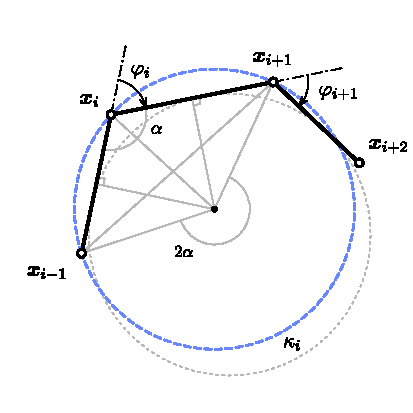
\includegraphics{kb_vertex.pdf}\label{fig:kb_vertex}}\hspace{5mm}
    		\subfloat[][edge-based]{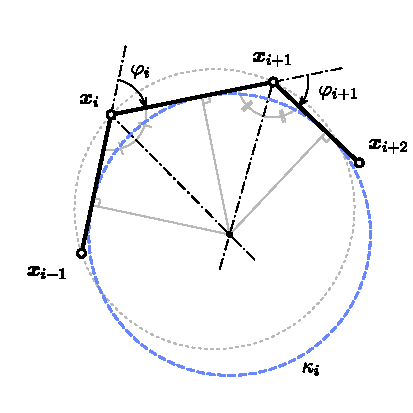
\includegraphics{kb_edge.pdf}\label{fig:kb_edge}} \\[-10pt]
		\subfloat[][bitangent with $\norm{\vect{e}_{i-1}}$]{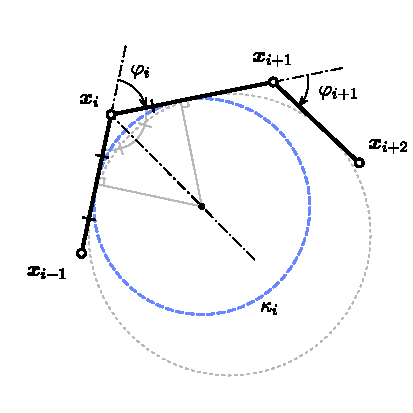
\includegraphics{kb_mixed_a.pdf}\label{fig:kb_mixed_a}}\hspace{5mm}
		\subfloat[][bitangent with $\norm{\vect{e}_{i}}$]{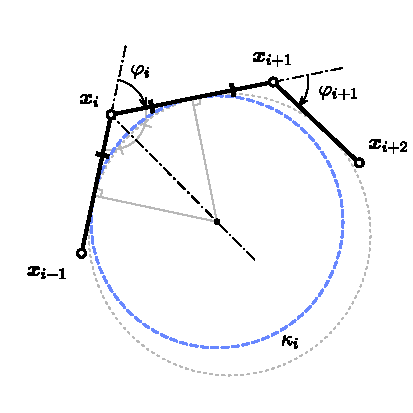
\includegraphics{kb_mixed_b.pdf}\label{fig:kb_mixed_b}}
		\vspace{10pt}
		\caption{Several ways to define the osculating circle for discrete curves, leading to different notions of discrete curvature.}
		\label{fig:kb_def}
   	\end{figure}
   	\begin{table}[h!] % not t or b or p
		\centering
      		% remaining contents of table environment
      		\renewcommand{\arraystretch}{1.5}
 		\begin{tabular}{l | c c c c c c}
      		\hline
		Curvature ($\kappa_i$) 										&  Locality 	&  $\varphi \mapsto 0$ 	&  $\varphi \mapsto \pi$ 		& Ends  	& Dim 	&  Fitting	\\
		\hline
		$\kappa_1 = \frac{2\, \sin(\varphi_i)}{\norm{\vect{e}_{i-1}+\vect{e}_i}}$ 	&  $\vect{x}_i$ 	&  $0$				&  $0, 2$					&  yes	&  space	&  clothoid		\\
		$\kappa_2 = \frac{\tan(\varphi_i/2)+\tan(\varphi_{i+1}/2)}{l_i}$ 			&  $\vect{e}_i$ 	&  $0$				&  $\infty$					&  no		&  planar	&  circle			\\
 		$\kappa_3 = \frac{2\, \tan(\varphi_i / 2)}{\overbar{l_i}} $				&  $\vect{x}_i$	&  $0$ 				&  $\infty$					&  no		&  space	&  circles			\\[5pt]
	\hline
		$\kappa_4 = \frac{2\,\sin(\varphi_i / 2)}{\overbar{l_i}}$ 				&  $\vect{x}_i$	&  $0$				&  $0, 2$					&  no		&  space	&  clothoid  		\\
		$\kappa_5 = \frac{\varphi_i}{\overbar{l_i}}$ 						&  $\vect{x}_i$	&  $0$				&  $\pi/\overbar{l_i}$			&  no		&  space	&  elastica  		\\[5pt]
		\hline
		\end{tabular}
		\caption{Review of several discrete curvature definitions mentioned in the literature.}
	\label{tab:kb_def}
   \end{table}
} % end of argument of `\afterpage` command


%\footnote{
%Curvature is defined from the osculating circle, which is the best approcximation of a curve by a circle.
%We can define such a circle and it's radius will be the curvature at that point. Problem : there are several ways to define such a circle.
%
%Très intéressant de constater que cette vision 3 verticies  vs. 2 edges est déjà présente dès le début dans l'histoire de la compréhension de la courbure.
%
%Pour Euler, le rayon de courbure est le rapport de l’élément d’arc sur l’angle de contin-
%gence entre deux tangentes infiniment proches. Par ailleurs, la définition du plan osculateur n’est pas tout à fait lamêmeque chez Bernoulli, plan passant par trois points consécutifs, puis- qu’Euler dit que ce plan contient deux éléments successifs. Il le définit aussi en disant que c’est le plan où la courbe s’incurve. Pour le dire de façon un peu différente : la tangente contient un élément, c’est le lieu où la courbe est droite, la plan osculateur représente l’étape suivante, c’est le lieu où la courbe est arc de cercle. Nous ne pensons pas trahir Euler en faisant cette présen- tation : cela justifie que, pour lui, il est naturel de se placer sur le plan osculateur pour calculer le rayon de courbure. \cite{Delcourt2007}
%
%
%The edge osculating circle.
%The vertex osculating circle.
%La localité est meilleur dans le cas du vertex-based discret osculating circle.
%Pour des anlges élevés, le edge-based discret osculating circle est plus pertinent.
%La courbure tend vers l'infini quand les 2 edges deviennent colineaires.
%
%La définition du plan osculateur est univoque dans le cas discret : c'est localement le plan défini par 2 edges consécutifs.
%
%Ce n'est pas le cas de la courbure qui perd son côté intrinsèque.
%
%courbure discrete dans le cas général
%}

% vertex-based curvature
% -------------------------------
\subsubsection{Vertex-based osculating circle (circumscribed)}\label{sec:circumscribed}
Let $\Gamma$ be a discrete curve parametrized by arc length. The \emph{vertex-based} (or circumscribed) osculating circle at vertex $\vect{x}_{i}$ is defined as the unique circle passing through the points $\vect{x}_{i-1}$, $\vect{x}_{i}$ and $\vect{x}_{i+1}$ (see \cref{fig:kb_vertex}). This circle leads to the following definition of the curvature : \footnote{This curvature is also known as the \emph{Menger curvature}.}
\begin{equation}
	\vect{\kappa b}_i = \frac{2 \, \vect{e}_{i-1} \times \vect{e}_{i}}{\norm{\vect{e}_{i-1}} \norm{\vect{e}_{i}} \norm{\vect{e}_{i-1} + \vect{e}_{i}} }
	\quad , \quad
	\kappa_i = \norm{\vect{\kappa b}_i} = \frac{2 \, \sin(\varphi_i)}{\norm{\vect{e}_{i-1} + \vect{e}_{i}}}
\label{eq:def_kb_vertex}
\end{equation}
This definition shows a good locality as the curvature is attached to the vertex $\vect{x}_{i}$, right in the place where it occurs on the discret curve. In addition, this definition leads to a natural local spline interpolation by the circumscribed osculating circle itself. This interpolation has the advantage to pass exactly through three vertices, to lie on the osculating plane and to share the same curvature as $\Gamma$ at $\vect{x}_{i}$. It also leads to a natural definition of the tangent vector at $\vect{x}_{i}$ (see \cref{sec:tangent}).

Moreover, while this definition is valid only on the current portion of $\Gamma$ ($i \in[1, n-1]$), it is straightforward extended to its endings ($i=0,1$), provided that a unit tangent vector $\vect{t}_{0}$ (respectively $\vect{t}_{n}$) is given at $\vect{x}_{0}$ (resp. $\vect{x}_{n}$), as the unique circle tangent to $\vect{t}_{0}$ (resp. $\vect{t}_{n}$) passing through $\vect{x}_0$ and $\vect{x}_1$ (resp. $\vect{x}_{n-1}$ and $\vect{x}_n$) :
\begin{equation}
	\vect{\kappa b}_0 = \frac{2 \, \vect{e}_{0} \times \vect{t}_{0}}{\norm{\vect{e}_{0}}^2} 
	\quad , \quad
	\vect{\kappa b}_n = \frac{2 \, \vect{t}_{n} \times \vect{e}_{n-1}}{\norm{\vect{e}_{n-1}}^2} 
\end{equation}
This property will be very profitable in the discrete beam model developed later in the manuscript. It is examined more in details in section \cref{sec:tangent} about the definition of the tangent vector.

However, there are some important drawbacks as the curvature is bounded to $[0,2]$ (see \cref{fig:kb_bench}). When the curve tends to kinks ($\varphi \mapsto \pi$), one would expect the curvature to diverge toward infinity, but instead it tends to a finite value equals to $0$ ($l_{i-1} \neq l_i$) or $2$ ($l_{i-1} = l_i$). This issue can be bypassed if the discretization is refined \textquote{enough}. A criterion is given in the next section (\cref{sec:}).

%This expression can be written in a more convenient way for futur comparisons :
%\begin{equation}
%	\kappa_1 = \frac{2}{\overbar{l_i}} \sin(\varphi_i / 2) \times \beta_i
%	\quad , \quad 
%	\beta_i = 
%%		\frac{\cos(\varphi_i/2)}{\sqrt{1 - \frac{l_{i-1} l_i}{\overbar{l_i} \overbar{l_i}}  \sin^2(\varphi_i/2)}} 
%%		\frac{1}{\sqrt{1 + (1 - \frac{l_{i-1} l_i}{\overbar{l_i} \overbar{l_i}}) \tan^2(\varphi_i/2)}} 
%		\left( 1 + (1 - \frac{l_{i-1} l_i}{\overbar{l_i} \overbar{l_i}}) \tan^2(\varphi_i/2) \right)^{-1/2}
%\end{equation}
%Note that $\beta_i = 1$ for a constant edge length curve ($l_{i-1} = l_i$).

% edge-based curvature
% ------------------------------
\subsubsection{Edge-based osculating circle (inscribed)}
Let $\Gamma$ be a discrete curve parametrized by arc length. The \emph{edge-based} osculating circle at edge $\vect{e}_{i}$ is defined as the unique circle tangent to the edges $\vect{e}_{i-1}$, $\vect{e}_{i}$ and $\vect{e}_{i+1}$ (see \cref{fig:kb_edge}).
\begin{equation}
	\kappa_i = \frac{\tan(\varphi_i/2) + \tan(\varphi_{i+1}/2)}{\norm{\vect{e}_{i}}}
\label{eq:def_kb_edge}
\end{equation}
This definition shows an appropriate behavior when the curve tends to kicks, as the radius of curvature tends to zero ($\tan \varphi/2 \mapsto \infty$), and when the curve tends to be a straight line, as the curvature tends to $0$ ($\tan \varphi/2 \mapsto 0$).

However, it needs $\Gamma$ to be planar which is by far to restrictive regarding our goal (the modeling of 3D slender beams). Finally, this way of defining the curvature is not as local as one would expect as it is defined relatively to the edge $\vect{e}_{i}$ but not where the turning occurs, at vertices.

% mixed approach
% ---------------------
\subsubsection{Bitangent osculating circle (inscribed)} \label{sec:inscribed}
Let $\Gamma$ be a discrete curve parametrized by arc length. Following \cite{Vouga2014} we define the curvature regrading the mean length $\overbar{l_i}$ attached to $\vect{x}_{i}$ as : \footnote{This definition is also presented in \cite{Bobenko2015, Carroll2014} but in the more restrictive case of constant edge length discrete curves ($l_i = cst$).}
\begin{equation}
	\vect{\kappa b}_i = \frac{2}{\overbar{l_i}} \left( \frac{\vect{e}_{i-1} \times \vect{e}_{i}}{\norm{\vect{e}_{i-1}} \norm{\vect{e}_{i}} + \vect{e}_{i-1} \cdot \vect{e}_{i}} \right)
	\quad , \quad
	\kappa_i = \norm{\vect{\kappa b}_i} = \frac{2}{\overbar{l_i}} \tan(\varphi_i/2)
\end{equation}
This other definition combines the good locality of the vertex-based approach (see \cref{eq:def_kb_vertex}) and the proper behavior at bounds of the edge-based approach (see \cref{eq:def_kb_edge}). Given two adjacent edges $\vect{e}_{i-1}$ and $\vect{e}_{i}$, there exist an infinite number of circles that are tangent to both edges (see \cref{fig:kb_mixed_a} and \cref{fig:kb_mixed_b} for two remarkable circles among them), which center points all lie on the $\varphi_i-\pi$ angle bisector line. The corresponding osculating circle, known as the \emph{inscribed} circle, is constructed to touch both $\vect{e}_{i-1}$ and $\vect{e}_{i}$ at distance $\overbar{l_i}$ from $\vect{x}_{i}$. In the case of a constant edge length discrete curve, this definition of the osculating circle merges to the circles proposed in \cref{fig:kb_mixed_a} and \cref{fig:kb_mixed_b}.

However, this definition still exhibits some drawbacks as there is no natural way to extend it to the end vertices $\vect{x}_{0}$ and $\vect{x}_{n-1}$. The lack of a natural interpolation spline that passes through vertices and that is in correlation to the osculating circle is also detrimental in the context of our application.

% mixed approach
% ---------------------
\subsubsection{Other definitions of osculating circles}
In the literature, one can find other definitions for the discrete curvature that also correspond to the definition of an osculating circle. All these definitions are summarized in \cref{tab:kb_def}. For further informations, the reader should refer to \cite{Carroll2014, Vouga2014, Bobenko2015, Romon2013}.

In particular, \cite{Vouga2014} details which discrete curvature definitions parallel which property of the smooth curvature. It remarks that there is no \textquote{free-lunch} as none of the proposed definition satisfies every properties of the smooth curvature.

%\note{
%Unlike the smooth case we can not reparameterize a curve. A discrete curve is parameterized by arc length or it is not \citep[p. 10]{Hoffmann2008}.
%
%Cette condition est extrêmement exigente $\norm{\vect{e}_{i}} = cst$. Elle est tenable pour des modèles de poutre non connectées (où le pas de disctrétisation peut-être choisi uniform) mais pour en cas de connexion. Ce point n'est pas éclairci dans les articles de Audoly.
%}

%\begin{figure}[t]
%     \subfloat[][vertex-based]{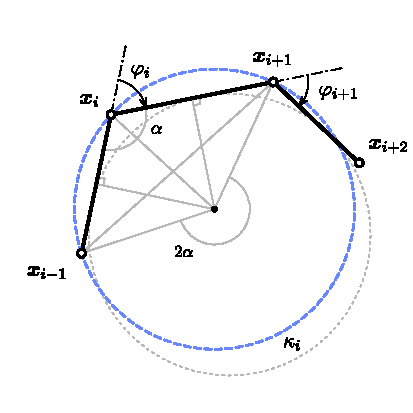
\includegraphics{kb_vertex.pdf}\label{fig:kb_vertex}}
%     \subfloat[][edge-based]{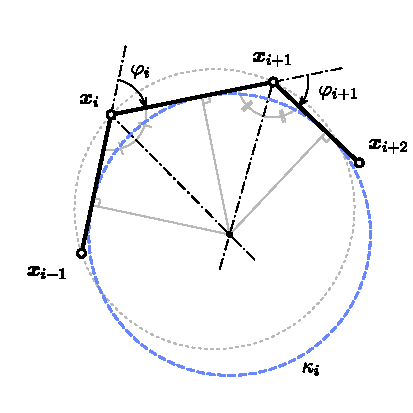
\includegraphics{kb_edge.pdf}\label{fig:kb_edge}}
%     \label{steady_state}
%     \centering
%     \caption{Main definition for the definition of the discrete osculating circle.}
%\end{figure}



%\begin{figure}[H]
%\begin{center}
%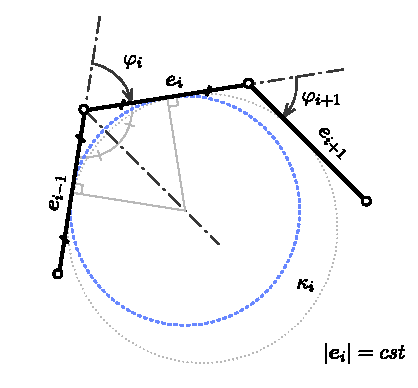
\includegraphics[]{osculating_circle_edge_cst.pdf}
%\caption{Another definition of the osculating circle for curve parametrized by arc lengths.}
%\label{fig:1_1}
%\end{center}
%\end{figure}



% sensitivity to non uniform discretization
% ----------------------------------------------------
\subsection{Benchmarking : sensitivity to non uniform discretization}
In this section we compare the two main discrete curvature notions (circumscribed versus inscribed) regarding their sensibility to non uniform discretization.

\begin{figure}[!p]
	\captionsetup[subfloat]{captionskip=10pt}
	\centering
	\vspace{-5mm}
	\subfloat[][vertex-based]{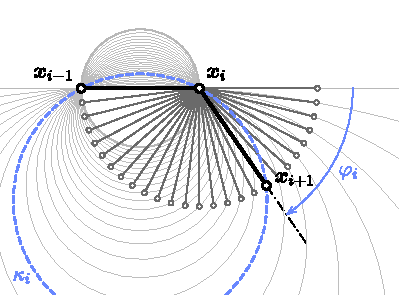
\includegraphics{kb_anim_vertex_a.pdf}\label{fig:1}}\hspace{5mm}
	\subfloat[][vertex-based]{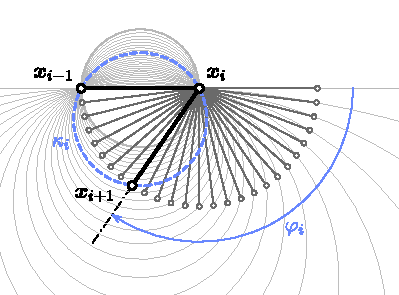
\includegraphics{kb_anim_vertex_b.pdf}\label{fig:2}} \\[-10mm]
	\subfloat[][edge-based]{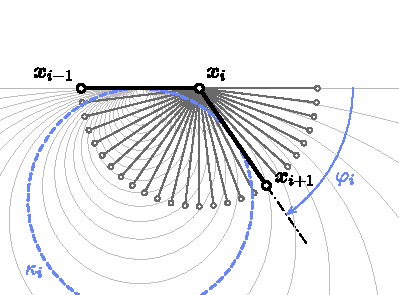
\includegraphics{kb_anim_edge_a.pdf}\label{fig:3}}\hspace{5mm}
	\subfloat[][edge-based]{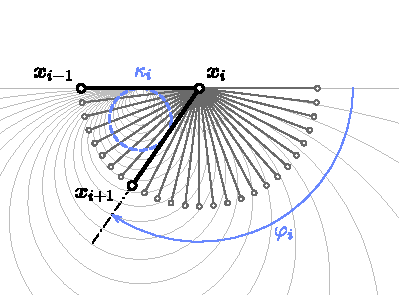
\includegraphics{kb_anim_edge_b.pdf}\label{fig:4}}
	\caption{Comparison of circumscribed (a-b) and inscribed (c-d) osculating circles for different values of the turning angle ($\varphi$).}
	\label{fig:kb_animation}
	\vspace{10mm}
	\begin{tikzpicture}
\begin{axis}[
	scale only axis,
	legend style={at={(axis cs:0,6)},anchor=north west},
	xmin=-3.1416/4/4, xmax= 3.1416+3.1416/4/4, restrict x to domain = 0 : 3.1416,
	ymin=-2/4, ymax= 10+2/4, restrict y to domain = 0 : 10,
	grid=major,
	axis y line*= left,% the '*' avoids arrow heads
%	xlabel={$\varphi$},
	xtick={0, 0.7854, 1.5708, 2.3562, 3.14159},
    	xticklabels={$0$, $\frac{\pi}{4}$,  $\frac{\pi}{2}$,  $\frac{3\pi}{4}$,$\pi$},
	ylabel={$\kappa_1, \kappa_3$},
	ytick={0, 2, 4, 6, 8,10} ]

		% kappa 1
		\addplot[black, samples = 100, domain = 0: 3.1416, solid,  thick]
		{2*sin(deg(x)/2)};
		\node[style={font=\scriptsize}] at (axis cs:3.0,2.4) {$\kappa_1$};
		\addplot[Tgray, samples = 100, domain = 0:3.1416, solid, very thin]					
		{\curvatureA(deg(x),2)};
		\addplot[color=Tgray, samples = 100, domain = 0:3.1416, solid, very thin]
		{\curvatureA(deg(x),0.5)};

		% kappa 2
		\addplot[black, samples = 400, domain = 0:3.1416, solid,  thick]
		{\curvatureB(deg(x),1)};
		\node[style={font=\scriptsize}] at (axis cs:3.0,9.5) {$\kappa_3$};
		\addplot[color=Tgray, samples = 400, domain = 0:3.1416, solid, very thin]
		{\curvatureB(deg(x),2)};
		\addplot[color=Tgray, samples = 400, domain = 0:3.1416, solid, very thin]
		{\curvatureB(deg(x),0.5)};


	\end{axis}
	\begin{axis}[
	scale only axis,
	xmin=-3.1416/4/4, xmax= 3.1416+3.1416/4/4, restrict x to domain = 0 : 3.1416,
	ymin=-0.2/4, ymax= 1+0.2/4, restrict y to domain = 0 : 1,
	axis y line*=right,
	axis x line=none,
%	ylabel style = {rotate=-90},
	ylabel = {${\kappa_1}/{\kappa_3}$},
	ytick={0, 0.2, 0.4, 0.6, 0.8, 1}
	]
		\addplot[Tblue, samples = 500, domain = 0:3.1416, solid, thick]
		{\curvatureRap(deg(x),1)};
		\node[style={font=\scriptsize}] at (axis cs:1.1,0.95) {$\kappa_1/\kappa_3$};
		\addplot[Tblue, samples = 500, domain = 0:3.1416, solid, very thin]
		{\curvatureRap(deg(x),2)};
	\end{axis}
\end{tikzpicture}

	\caption{Sensitivity of discrete curvatures to non uniform discretization ($\alpha \in [0.5,2]$) over the whole domain of variation of the turning angle ($\varphi \in [0,\pi]$).}
	\label{fig:kb_bench}
\end{figure}

This aspect is not treated in the actual literature, in which curves parametrized by arc length are usually treated as curves of constant edge length, though it is yet an important topic when it comes to the numerical modeling of true mechanical systems. Indeed, the presence of connexions between members will compromise the ability to enforce a constant discretization through all the elements of the structure. Additionally, vertices are obviously points of interest in a discrete model as they will be used to apply loads and enforce various constraints such as joints and support conditions. Finally, the accuracy of the discretized model is proportional to the sharpness of the discretization, whereas the computing time required to solve the model will grow as the sharpness increases. Consequently, one would distribute those points in the space as cleverly as possible and try to minimize their number as they increase the overall computation cost.

Introducing the coefficient $\alpha = \frac{\norm{\vect{e}_{i-1}}}{\norm{\vect{e}_{i}}}$, we rewrite the previous formulas for $\kappa_1$ and $\kappa_3$ as :
\begin{equation}
\begin{aligned}
	\kappa_1 &= \frac{2 \,\sin(\varphi)}{\norm{\vect{e}_{i}}(1+ \alpha^2 + 2 \alpha \, \cos(\varphi))^{1/2}} \\[10pt]
	\kappa_3 &= \frac{4 \,\tan(\varphi/2)}{\norm{\vect{e}_{i}}(1+\alpha)}
\end{aligned}
\end{equation}
These expressions lead to the following formula for the ratio $\kappa_1 / \kappa_3$, which relies only on $\alpha$ and the turning angle $\varphi$ between the edges $\vect{e}_{i-1}$ and $\vect{e}_{i}$ :
\begin{equation}
	\frac{\kappa_1}{\kappa_3}(\alpha) = \frac{\kappa_1}{\kappa_3}(1/\alpha)= \frac{(1+\alpha)\,cos^2(\varphi/2)}{((1- \alpha)^2 + 4 \alpha \, cos^2(\varphi/2))^{1/2}}
	\label{eq:ratio_inv}
\end{equation}
Discrete curvatures are plotted in \cref{fig:kb_bench} for three values of $\alpha$. The thickest line is for the case of uniform discretization ($\alpha=1$), whereas the thin lines mark the boundary cases ($\alpha=0.5,2$). The ratio $\kappa_1/\kappa_3$ is plotted in blue and leads to only one thin line (remind \cref{eq:ratio_inv}). The graph shows that $\kappa_1$ and $\kappa_3$ have a very close behavior for small turning angles. The variability regarding $\alpha$ is small when $\varphi$ remains small and gets negligible as $\varphi$ gets smaller.

Passing $\pi/4$ and increasing $\varphi$, $\kappa_3$ exhibits a good behavior : as the discrete curves tends to kink $\kappa_3$ diverges towards the infinity as the smooth curvature would for  




However, for a given curvature, the turning angle decreases as the sharpness of the discretization increases ($\lim_{\norm{\vect{e}_i} \mapsto 0} \varphi_i = 0$). Thus, it is possible to adapted the discretization to make sure

% DOUBLE PAGE SIDE BY SIDE FIGURES
\begin{figure}[!p]
\begin{leftfullpage}
	\captionsetup[subfloat]{captionskip=10pt}
	\centering
%	\vspace{-5mm}
	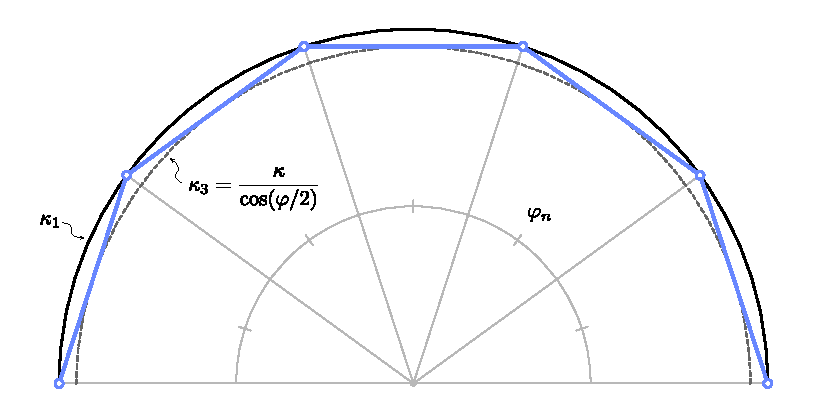
\includegraphics[]{semicircle.pdf}
	\caption{Discretization of a semicircle for discrete bending energies evaluation.}
	\label{fig:semicircle}
	\vspace{10mm}
	\subfloat[][$| 1-\frac{\mathcal{E}_1}{\mathcal{E}}(n) |$ in \%]{\begin{tikzpicture}
	\begin{axis}[
	width = 7.5cm,
	xmin=3, xmax= 52, restrict x to domain = 5 : 50,
	ymin=-0.5, ymax= 10.5, restrict y to domain = 0:100,
	grid=major,
	xtick={0,5,10,15,20,25,30,35,40,45,50},
	ytick={0,2,4,6,8,10},
	]
%		\addplot[black, very thin, samples = 10, domain = 10: 50]
%		{sin(deg(pi/(2*x))/(pi/(2*x))};

		\pgfplotstableread{ch3_geometry/plot/semicircle/semicircle.txt}\crvC;
		\addplot [Tblue, smooth, thin]
        		table [x expr=\thisrowno{0}, y expr=\thisrowno{6}] {\crvC};

%		\addplot[Tblue, samples = 50, domain = 10: 50, solid,  thick]
%		{1};
%		 			
	\end{axis}
\end{tikzpicture}

		\label{plot:bench_semicircle_vertex}}\hspace{5mm}
	\subfloat[][$| 1-\frac{\mathcal{E}_3}{\mathcal{E}}(n) |$ in \%]{\begin{tikzpicture}
	\begin{axis}[
	width = 7.5cm,
	xmin=3, xmax= 52, restrict x to domain = 5 : 50,
	ymin=-0.5, ymax= 10.5, restrict y to domain = 0:100,
	grid=major,
	xtick={0,5,10,15,20,25,30,35,40,45,50},
	ytick={0,2,4,6,8,10},
	]
%		\addplot[black, smooth, very thin, solid, samples = 50, domain = 10: 50]
%		{sin(deg(pi/(2*x)))/((pi/(2*x))*cos(deg(pi/(2*x)))^2)};
%		\node[style={font=\scriptsize}] at (axis cs:2.5,0.65) {$\mathcal{E}_3/\mathcal{E}$};

		\pgfplotstableread{ch3_geometry/plot/semicircle/semicircle.txt}\crvC;
		\addplot [Tblue, smooth, thin]
        		table [x expr=\thisrowno{0}, y expr=\thisrowno{7}] {\crvC};

%		\addplot[Tblue, samples = 50, domain = 10: 50, solid,  thick]
%		{1};
%			
	\end{axis}
\end{tikzpicture}

		\label{plot:bench_semicircle_vertex}}
	\vspace{8pt}
	\caption{Relative error in the estimation of the smooth bending energy ($\mathcal{E}$) by the discrete bending energies ($\mathcal{E}_1$ and $\mathcal{E}_3$) regarding the sharpness of the discretization, for a semicircle.}
	\label{fig:bench_semicircle}
\end{leftfullpage}
\end{figure}
\begin{figure}[!p]
\begin{fullpage}
	\captionsetup[subfloat]{captionskip=10pt}
	\centering
%	\vspace{-5mm}
	\subfloat[][sequence of elastica curves]{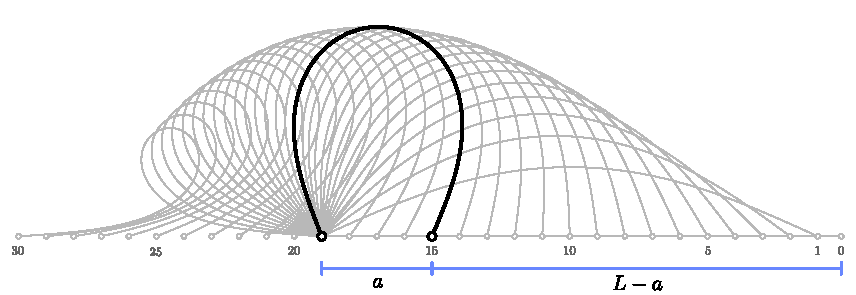
\includegraphics{elastica.pdf}\label{fig:elastica_seq}}\\[5mm]
	\subfloat[][zoom on the discretization]{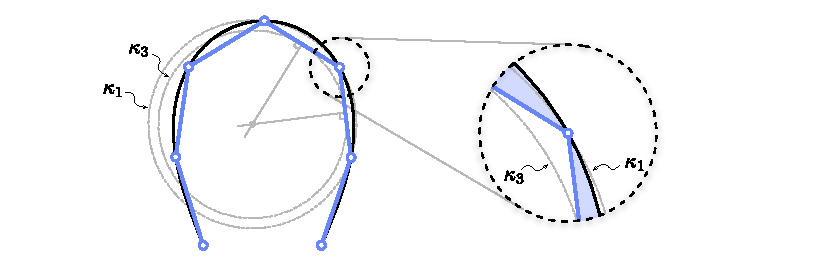
\includegraphics{elastica_zoom.pdf}\label{fig:elastica_discretization}}
	\vspace{12pt}
	\caption{Discretization (b) of a sequence of elastica curves (a) for discrete bending energies evaluation.}
	\label{fig:elastica}
	\vspace{10mm}
	\subfloat[][$|1-\frac{\mathcal{E}_1}{\mathcal{E}}(n) |$ in \%]{\begin{tikzpicture}
\begin{axis}[
	width = 7.5cm,
	xmin=3, xmax= 52, restrict x to domain = 5 : 50,
	ymin=-0.5, ymax= 10.5, restrict y to domain = 0 :100,
	grid=major,
	xtick={0,5,10,15,20,25,30,35,40,45,50},
	ytick={0,2,4,6,8,10},
	]
	
	\pgfplotstableread{ch3_geometry/plot/elastica/elastica_1.txt}\crvA;
	\addplot [Tblue, smooth, thin]
       	table [x expr=\thisrowno{0}, y expr=\thisrowno{6}] {\crvA};
  	\node[Tgray, style={font=\scriptsize}] at (axis cs:7.5,1) {$1$};
	
	\pgfplotstableread{ch3_geometry/plot/elastica/elastica_5.txt}\crvB;
	\addplot [Tblue, smooth, thin]
       	table [x expr=\thisrowno{0}, y expr=\thisrowno{6}] {\crvB};
%  	\node[Tgray, style={font=\scriptsize}] at (axis cs:9,1) {$5$};

       	\pgfplotstableread{ch3_geometry/plot/elastica/elastica_10.txt}\crvC;
	\addplot [Tblue, smooth, thin]
        	table [x expr=\thisrowno{0}, y expr=\thisrowno{6}] {\crvC};
%    	\node[Tgray, style={font=\scriptsize}] at (axis cs:10,0.985) {$10$};

        \pgfplotstableread{ch3_geometry/plot/elastica/elastica_15.txt}\crvD;
	\addplot [Tblue, smooth, thin]
         table [x expr=\thisrowno{0}, y expr=\thisrowno{6}] {\crvD};
%         \node[Tgray, style={font=\scriptsize}] at (axis cs:10,0.978) {$15$};

     	\pgfplotstableread{ch3_geometry/plot/elastica/elastica_20.txt}	\crvE;
	\addplot [Tblue, smooth, thin]
       	table [x expr=\thisrowno{0}, y expr=\thisrowno{6}] {\crvE};
%       	\node[Tgray, style={font=\scriptsize}] at (axis cs:10,0.965) {$20$};

     	\pgfplotstableread{ch3_geometry/plot/elastica/elastica_25.txt}	\crvF;
	\addplot [Tblue, smooth, thin]
       	table [x expr=\thisrowno{0}, y expr=\thisrowno{6}] {\crvF};
%       	\node[Tgray, style={font=\scriptsize}] at (axis cs:10,0.94) {$25$};

     	\pgfplotstableread{ch3_geometry/plot/elastica/elastica_30.txt}	\crvG;
	\addplot [Tblue, smooth, thin]
        	table [x expr=\thisrowno{0}, y expr=\thisrowno{6}] {\crvG};
       	\node[Tgray, style={font=\scriptsize}] at (axis cs:17.5,7) {$30$};
	
	
%	
%
%       	\pgfplotstableread{ch3_geometry/plot/discrete_curvature_bench/elastica5.txt}\crvB;
%	\addplot [black, smooth, thin]
%       	table [x expr=\thisrowno{0}, y expr=\thisrowno{3}] {\crvB};
%  	\node[Tgray, style={font=\scriptsize}] at (axis cs:9,1) {$5$};
%
%       	\pgfplotstableread{ch3_geometry/plot/discrete_curvature_bench/elastica10.txt}\crvC;
%	\addplot [black, smooth, thin]
%        	table [x expr=\thisrowno{0}, y expr=\thisrowno{3}] {\crvC};
%    	\node[Tgray, style={font=\scriptsize}] at (axis cs:10,0.985) {$10$};
%
%        \pgfplotstableread{ch3_geometry/plot/discrete_curvature_bench/elastica15.txt}\crvD;
%	\addplot [black, smooth, thin]
%         table [x expr=\thisrowno{0}, y expr=\thisrowno{3}] {\crvD};
%         \node[Tgray, style={font=\scriptsize}] at (axis cs:10,0.978) {$15$};
%
%     	\pgfplotstableread{ch3_geometry/plot/discrete_curvature_bench/elastica20.txt}	\crvE;
%	\addplot [black, smooth, thin]
%       	table [x expr=\thisrowno{0}, y expr=\thisrowno{3}] {\crvE};
%       	\node[Tgray, style={font=\scriptsize}] at (axis cs:10,0.965) {$20$};
%
%     	\pgfplotstableread{ch3_geometry/plot/discrete_curvature_bench/elastica25.txt}	\crvF;
%	\addplot [black, smooth, thin]
%       	table [x expr=\thisrowno{0}, y expr=\thisrowno{3}] {\crvF};
%       	\node[Tgray, style={font=\scriptsize}] at (axis cs:10,0.94) {$25$};
%
%     	\pgfplotstableread{ch3_geometry/plot/discrete_curvature_bench/elastica30.txt}	\crvG;
%	\addplot [black, smooth, thin]
%        	table [x expr=\thisrowno{0}, y expr=\thisrowno{3}] {\crvG};
%       	\node[Tgray, style={font=\scriptsize}] at (axis cs:15,0.92) {$30$};

%         \addplot[Tblue, samples = 100, domain = 0: 50, solid,  thick]
%	{1};
	
\end{axis}
\end{tikzpicture}
		\label{plot:bench_elastica_vertex}}\hspace{5mm}
	\subfloat[][$| 1-\frac{\mathcal{E}_3}{\mathcal{E}}(n) |$ in \%]{\begin{tikzpicture}
\begin{axis}[
	width = 7.5cm,
	xmin=3, xmax= 52, restrict x to domain = 5 : 50,
	ymin=-0.5, ymax= 10.5, restrict y to domain = 0:100,
	grid=major,
	xtick={0,5,10,15,20,25,30,35,40,45,50},
	ytick={0,2,4,6,8,10},
	]
	
         \pgfplotstableread{ch3_geometry/plot/elastica/elastica_1.txt}\crvA;
	\addplot [Tblue, smooth, thin]
         table [x expr=\thisrowno{0}, y expr=\thisrowno{7}] {\crvA};
         \node[Tgray, style={font=\scriptsize}] at (axis cs:7.5,1.0) {$1$};
	
	% celle la pose probleme. problem dans le script rhino a regarder.
%	\pgfplotstableread{ch3_geometry/plot/elastica/elastica_5.txt}\crvB;
%	\addplot [red, smooth, thin]
%         table [x expr=\thisrowno{0}, y expr=\thisrowno{7}] {\crvB};
%         \node[Tgray, style={font=\scriptsize}] at (axis cs:10,1.024) {$5$};

        \pgfplotstableread{ch3_geometry/plot/elastica/elastica_10.txt}\crvC;
	\addplot [Tblue, smooth, thin]
         table [x expr=\thisrowno{0}, y expr=\thisrowno{7}] {\crvC};
%         \node[Tgray, style={font=\scriptsize}] at (axis cs:10,1.044) {$10$};

         \pgfplotstableread{ch3_geometry/plot/elastica/elastica_15.txt}\crvD;
	\addplot [Tblue, smooth, thin]
         table [x expr=\thisrowno{0}, y expr=\thisrowno{7}] {\crvD};
%         \node[Tgray, style={font=\scriptsize}] at (axis cs:10,1.07) {$15$};

     	\pgfplotstableread{ch3_geometry/plot/elastica/elastica_20.txt}	\crvE;
	\addplot [Tblue, smooth, thin]
         table [x expr=\thisrowno{0}, y expr=\thisrowno{7}] {\crvE};
%         \node[Tgray, style={font=\scriptsize}] at (axis cs:13.5,1.08) {$20$};

     	\pgfplotstableread{ch3_geometry/plot/elastica/elastica_25.txt}	\crvF;
	\addplot [Tblue, smooth, thin]
         table [x expr=\thisrowno{0}, y expr=\thisrowno{7}] {\crvF};
%         \node[Tgray, style={font=\scriptsize}] at (axis cs:16,9.70) {$25$};

     	\pgfplotstableread{ch3_geometry/plot/elastica/elastica_30.txt}	\crvG;
	\addplot [Tblue, smooth, thin]
         table [x expr=\thisrowno{0}, y expr=\thisrowno{7}] {\crvG};
         \node[Tgray, style={font=\scriptsize}] at (axis cs:28.5,7) {$30$};

%
%         \pgfplotstableread{ch3_geometry/plot/discrete_curvature_bench/elastica5.txt}\crvB;
%	\addplot [black, smooth, thin]
%         table [x expr=\thisrowno{0}, y expr=\thisrowno{4}] {\crvB};
%         \node[Tgray, style={font=\scriptsize}] at (axis cs:10,1.024) {$5$};
%
%        \pgfplotstableread{ch3_geometry/plot/discrete_curvature_bench/elastica10.txt}\crvC;
%	\addplot [black, smooth, thin]
%         table [x expr=\thisrowno{0}, y expr=\thisrowno{4}] {\crvC};
%         \node[Tgray, style={font=\scriptsize}] at (axis cs:10,1.044) {$10$};
%
%         \pgfplotstableread{ch3_geometry/plot/discrete_curvature_bench/elastica15.txt}\crvD;
%	\addplot [black, smooth, thin]
%         table [x expr=\thisrowno{0}, y expr=\thisrowno{4}] {\crvD};
%         \node[Tgray, style={font=\scriptsize}] at (axis cs:10,1.07) {$15$};
%
%     	\pgfplotstableread{ch3_geometry/plot/discrete_curvature_bench/elastica20.txt}	\crvE;
%	\addplot [black, smooth, thin]
%         table [x expr=\thisrowno{0}, y expr=\thisrowno{4}] {\crvE};
%         \node[Tgray, style={font=\scriptsize}] at (axis cs:13.5,1.08) {$20$};
%
%     	\pgfplotstableread{ch3_geometry/plot/discrete_curvature_bench/elastica25.txt}	\crvF;
%	\addplot [black, smooth, thin]
%         table [x expr=\thisrowno{0}, y expr=\thisrowno{4}] {\crvF};
%         \node[Tgray, style={font=\scriptsize}] at (axis cs:18,1.08) {$25$};
%
%     	\pgfplotstableread{ch3_geometry/plot/discrete_curvature_bench/elastica30.txt}	\crvG;
%	\addplot [black, smooth, thin]
%         table [x expr=\thisrowno{0}, y expr=\thisrowno{4}] {\crvG};
%         \node[Tgray, style={font=\scriptsize}] at (axis cs:27,1.08) {$30$};

%         \addplot[Tblue, samples = 100, domain = 0: 50, solid,  thick]
%	{1};

\end{axis}
 \end{tikzpicture}

		\label{plot:bench_elastica_vertex}}
	\vspace{8pt}
	\caption{Relative error in the estimation of the smooth bending energy ($\mathcal{E}$) by the discrete bending energies ($\mathcal{E}_1$ and $\mathcal{E}_3$) regarding the sharpness of the discretization, for several elastica curves. The curves are chosen from \cref{fig:elastica_seq} (1,5,10,15,20,25,30).}
	\label{fig:bench_elastica}
\end{fullpage}
\end{figure}


% accuracy in bending energy representation
% ---------------------------------------------------------
\subsection{Benchmarking : accuracy in bending energy representation}

In this section we compare, for three remarkable types of curves (line, semicircle and elastica), the discrete bending energies $\mathcal{E}_1$ and $\mathcal{E}_3$ of the discrete curve, respectively based on definitions $\kappa_1$ and $\kappa_3$ (see \cref{tab:kb_def}), to the bending energy $\mathcal{E}$ of the smooth curve. We study the convergence of these energies as the sharpness of the discretization increases. The energies are defined as :
\begin{equation}
\setlength{\jot}{8pt}
\begin{aligned}
	\mathcal{E} &= \int_0^L \kappa^2 ds\\
	\mathcal{E}_i &= \sum_i \overbar{l_i} \kappa_i^2
\end{aligned}
\end{equation}

% Straight line
\subsubsection{Straight line}

We consider any straight line. Its smooth curvature is null. So are the discrete curvatures $\kappa_1$ and $\kappa_3$ (see \cref{tab:kb_def}). In this case, the discrete bending energies perfectly match the bending energy of the smooth curve :
\begin{equation}
	\mathcal{E} = \mathcal{E}_1 = \mathcal{E}_3 = 0
\end{equation}

% Circle
\subsubsection{Semicircle}

We consider a semicircle of curvature $\kappa =1/r$ and length $L = \pi r$. This curve is discretized into $n$ edges of equal length $|\vect{e}_n| = 2r\sin (\varphi/2)$ where $\varphi = \tfrac{\pi}{n}$ (see \cref{fig:semicircle}). The total length of the discrete curve is given by : $L_n = n |\vect{e}_n| = L \frac{\sin(\varphi/2)}{\varphi/2}$. In this simple case, the bending energies can be expressed analytically :
\begin{subequations}
\setlength{\jot}{6pt}
\begin{alignat}{5}
	&\mathcal{E}		& = && \,	&	L \kappa^2		&	&&	&	\\
	&\mathcal{E}_1		& = && 	&	L_n  \kappa_1^2 	& = 	&& \,	&	\frac{\sin (\varphi/2)}{\varphi/2} \cdot \mathcal{E}  \\
	&\mathcal{E}_3	\,	& = && 	& 	L_n  \kappa_3^2 \, 	&= 	&&	& 	\frac{\sin (\varphi/2)}{(\varphi/2) \cos^2 (\varphi/2)} \cdot \mathcal{E} 
\end{alignat}
\end{subequations}
Note that $\kappa_1$ equals the curvature of the smooth curve. Consequently, the estimation error is only due to the estimation of the curve length ($L_n \neq L$). The ratios $\mathcal{E}_1/\mathcal{E}$ and $\mathcal{E}_3/\mathcal{E}$ are plotted in \cref{fig:bench_semicircle}. Graphs show that $\mathcal{E}_1$ converges to the smooth case faster than $\mathcal{E}_3$.

% Elastica
\subsubsection{Elastica}
We consider a sequence of elastica curves of fixed length $L$ and variable curvature $\kappa$ (see \cref{fig:elastica_seq}). This curves correspond to a buckled shape of a straight pinned-pinned beam that would have been forced to retract its span. These curves are discretized into $n$ edges of equal length (see \cref{fig:elastica_discretization}). This time, there is no analytical expressions available for $\mathcal{E}$, $\mathcal{E}_1$ and $\mathcal{E}_3$. Results are obtained by numerical integration and plotted in \cref{fig:bench_elastica}. Again, graphs show that $\mathcal{E}_1$ converges to the smooth case faster than $\mathcal{E}_3$ for most of the curves excepted the ones with low overall curvature (1 to 5).

% DISCRETE TANGENT VECTOR
% ===================
\section{Discrete tangent vector}\label{sec:tangent}

In this section we study how to define the discrete unit tangent vector relative to a discrete curve. While a natural definition exists along the edges (see \cref{sec:tangent_edge}, there is no obvious choice at vertices were the curve kinks.

The ability to define a unique tangent vector is very important to define the normal to cross section, control beam endings, and relate it to curvature.
You will controle the directiopn of the section (for a fixed/encastre support condition) or inversly, you would control the moment and seek the corresponding tangent direction (for a pin boundary condition, you know there is no end moments so the curvature is null and your looking for the tangent).

Problème de définition. Facile de définir une tangente sur un edge. Mais une infinité de tangentes possibles à chaque vertex. So in case of an arc length parameterized curve the vertex tangent vector points in the same direction as the averaged edge tangent vectors \cite[p.12]{Hoffmann2008}. Nous verrons que le cercle 3 points, en plus de mieux représenter l'énergie d'une courbe discrete dans les cas typiques, offre un choix de tangente non ambïgu.

\subsection{Circumscribed case}

We consider the case where the curvature is defined according to the circumscribed osculating circle (see \cref{fig:kb_vertex_tangent_a}). 

\subsubsection{Current portion}

Let $\vect{x}_i$ be a vertex in the current portion of $\Gamma$. The circumscribed osculating circle gives a smooth approximation of $\Gamma$ in the vicinity of $\vect{x}_i$ (see \cref{fig:kb_vertex_tangent_a}). It leads to a natural definition of a unit tangent vector for five remarkable vertices as the tangent to the osculating circle at those points (resp. $\vect{x}_{i-1}$, $\vect{x}_{i-1/2}$, $\vect{x}_i$,  $\vect{x}_{i+1/2}$, $\vect{x}_{i+1}$) : 
\begin{subequations}
\setlength{\jot}{6pt}
\begin{alignat}{4}
	&\vect{t}_i^- 		& \quad 	&= 	 \quad 	&&2 (\vect{t}_{i} \cdot \vect{u}_{i-1}) \vect{u}_{i-1} - \vect{t}_{i}  				&\hspace{10mm}	& \\
	&\vect{t}_{i-1/2} 	& 		&=	 		&&\vect{u}_{i-1}  												&				& \\
	&\vect{t}_i 		& 		&=	 		&&\frac{\norm{\vect{e}_{i}}}{\norm{\vect{e}_{i-1} + \vect{e}_{i}}} \vect{u}_{i-1}	
				 					+ 	\frac{\norm{\vect{e}_{i-1}}}{\norm{\vect{e}_{i-1} + \vect{e}_{i}}} \vect{u}_{i} 		&				& \\
	&\vect{t}_{i+1/2} 	& 		&=	 		&&\vect{u}_{i}  													&				& \\
	&\vect{t}_i^+ 		& 		&= 	 		&&2 (\vect{t}_{i} \cdot \vect{u}_{i}) \vect{u}_{i} - \vect{t}_{i}					&				&
\end{alignat}
\end{subequations}
Note that $\vect{t}_i^-$ (resp. $\vect{t}_i^+$) is obtained by a reflection of $-\vect{t}_i$ across the bisecting plane of $\vect{e}_{i-1}$ (resp. $\vect{e}_{i}$).  A very important property is that the curvature binormal vector at $\vect{x}_i$ can be computed by three different ways :
\begin{equation}
	\vect{\kappa b}_{i} =  \frac{2 \, \vect{e}_{i-1} \times \vect{e}_{i}}{\norm{\vect{e}_{i-1}} \norm{\vect{e}_{i}} \norm{\vect{e}_{i-1} + \vect{e}_{i}} }
	=
	\left \{
	\begin{aligned}	
		& \frac{2\,\vect{u}_{i-1} \times  \vect{t}_{i} }{\norm{\vect{e}_{i-1}}} 
%		= \frac{2}{\norm{\vect{e}_{i-1}}} \vect{t}_{i-1} \times  \vect{u}_{i-1}
		\\[8pt]
		& \frac{2\, \vect{t}_{i} \times  \vect{u}_{i}}{\norm{\vect{e}_{i}}}
%		= \frac{2}{\norm{\vect{e}_{i}}} \vect{u}_{i} \times  \vect{t}_{i+1} 
	\end{aligned}
	\right.
\label{eq:vertex_kbs}
\end{equation}
The first expression is interpreted as the unique circle passing through three points ($\vect{x}_{i-1}$, $\vect{x}_i$, $\vect{x}_{i+1}$) as explained in \cref{sec:circumscribed}. Equivalently, there exist a unique circle defined by two points and a tangent vector. Precisely, the last two expressions in \cref{eq:vertex_kbs} can be interpreted as the curvature binormal vector of the unique circle passing through $\vect{x}_{i-1}$, $\vect{x}_i$ (resp. $\vect{x}_{i}$, $\vect{x}_{i+1}$) and tangent to $\vect{t}_{i}$ at $\vect{x}_{i}$.

\begin{figure}[p]
	\captionsetup[subfloat]{captionskip=20pt}
	\centering
	\subfloat[][current portion]{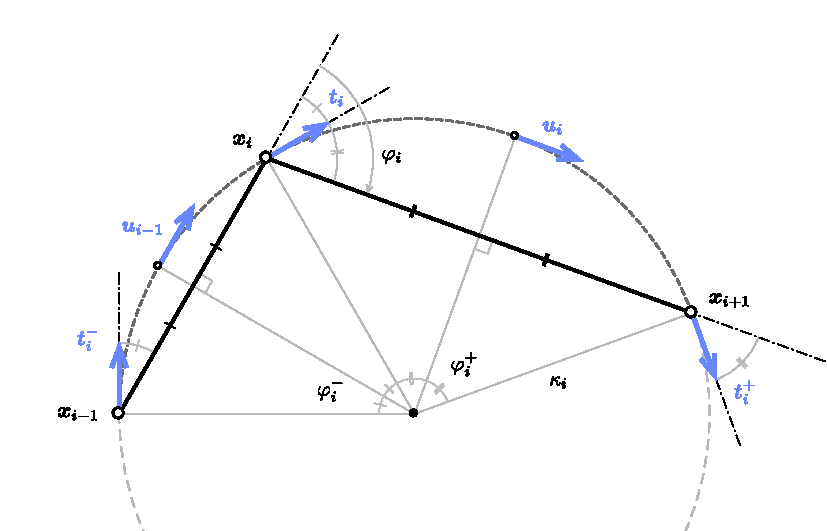
\includegraphics{kb_vertex_tangent.pdf}\label{fig:kb_vertex_tangent_a}}\\
	\subfloat[][start]{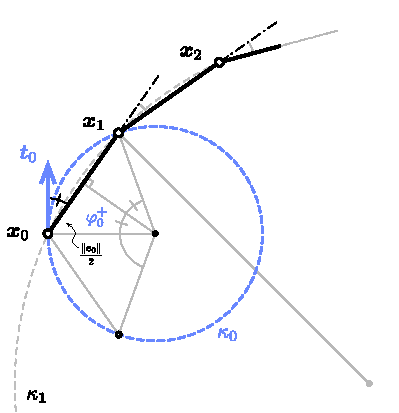
\includegraphics{kb_vertex_start.pdf}\label{fig:kb_vertex_tangent_b}}\hspace{5mm}
	\subfloat[][end]{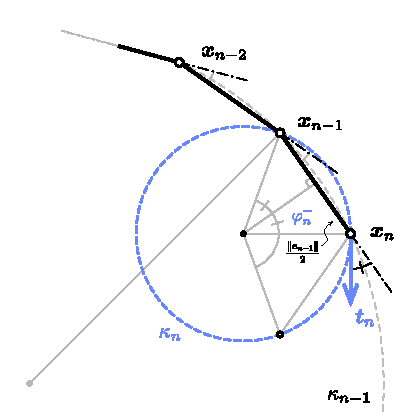
\includegraphics{kb_vertex_end.pdf}\label{fig:kb_vertex_tangent_c}}
	\vspace{10pt}
	\caption{Definition of the tangent vector ($\vect{t}$) and related curvature binormal vector ($\vect{\kappa b}$) at vertices (circumscribed definition).}
	\label{fig:kb_vertex_tangent}
\end{figure}

\subsubsection{Discontinuity of curvature}
Let $\vect{t}_i^*$ be an arbitrary tangent vector at $\vect{x}_i$. Following \cref{eq:vertex_kbs} we define the \emph{left-sided} (resp. \emph{right-sided}) discrete curvatures at $\vect{x}_i$ in the circumscribed case as :
\begin{subequations}as
\setlength{\jot}{8pt}
\begin{alignat}{2}
	&\vect{\kappa b}_{i}^-(\vect{t}_i^*) 	&&=  \frac{2\,\vect{u}_{i-1} \times  \vect{t}_{i}^* }{\norm{\vect{e}_{i-1}}} \\
%	&\vect{\kappa b}_{i} 		&&=  \frac{2 \, \vect{e}_{i-1} \times \vect{e}_{i}}{\norm{\vect{e}_{i-1}} \norm{\vect{e}_{i}} \norm{\vect{e}_{i-1} + \vect{e}_{i}} } \\
	&\vect{\kappa b}_{i}^+(\vect{t}_i^*)	&&=  \frac{2\, \vect{t}_{i}^* \times  \vect{u}_{i}}{\norm{\vect{e}_{i}}}
\end{alignat}
\end{subequations}
The corresponding osculating circle will be called the \emph{left-sided} (resp. \emph{right-sided}) circumscribed osculating circle. When $\vect{t}_i^* = \vect{t}_i$, the limits agree one to each other ($\vect{\kappa b}_{i}^- = \vect{\kappa b}_{i}^+ = \vect{\kappa b}_{i}$) and the osculating circles coincide. These definitions perfectly mimic the smooth case where, at a regular ($\norm{\gamma'} \neq 0$) but not biregular ($\norm{\gamma''} = 0$) point, the curvature is discontinuous while the tangent vector reminds smoothly defined.

In mechanics, this situation is likely to arise as discontinuities in material properties or punctual applied moments will necessarily lead to discontinuities in curvature (recall that $M = EI\kappa$).

\subsubsection{Curve endings}
The definition of the left and right sided curvatures given for a vertex in the current portion of $\Gamma$ are still valid for the end vertices $\vect{x}_{0}$ and $\vect{x}_{n}$. Provided that a unit tangent vector $\vect{t}_{0}^*$ (respectively $\vect{t}_{n}^*$) is given at $\vect{x}_{0}$ (resp. $\vect{x}_{n}$), the circumscribed osculating circle is defined as the unique circle passing through $\vect{x}_0$ and $\vect{x}_1$ (resp. $\vect{x}_{n-1}$ and $\vect{x}_n$) tangent to $\vect{t}_{0}^*$ (resp. $\vect{t}_{n}^*$) ; see \cref{fig:kb_vertex_tangent_b} and \cref{fig:kb_vertex_tangent_c}. It leads to the following curvature binormal vectors :
\begin{subequations}
\setlength{\jot}{8pt}
\begin{alignat}{2}
	&\vect{\kappa b}_0 =\vect{\kappa b}_{0}^+(\vect{t}_0^*)	&&=  \frac{2\, \vect{t}_{0}^* \times \vect{e}_{0} }{\norm{\vect{e}_{0}}^2} \\
	&\vect{\kappa b}_n =\vect{\kappa b}_{n}^-(\vect{t}_n^*) 	&&=  \frac{2\, \vect{e}_{n-1} \times  \vect{t}_{n}^*}{\norm{\vect{e}_{n-1}}^2} 
\end{alignat}
\end{subequations}
Note that, contrary to the current portion, curvatures at endings are subjected to the definition of a unit tangent vector. This reflects the usual indetermination of boundary conditions. For a given beam whether the end is clamped, the tangent vector is known and one will seek the reacting moment due to the support ; whether the end is pinned, the reacting moment is null (so is the curvature) and one will seek the cross section orientation.

\subsection{Inscribed case}

We now consider the case where the curvature is defined according to the inscribed osculating circle (see \cref{fig:kb_edge_tangent_a}). Remark that inscribed and circumscribed osculating circles are concentric when $l_{i-1} = l_i$.

\begin{figure}[p]
	\captionsetup[subfloat]{captionskip=20pt}
	\centering
	\subfloat[][current portion]{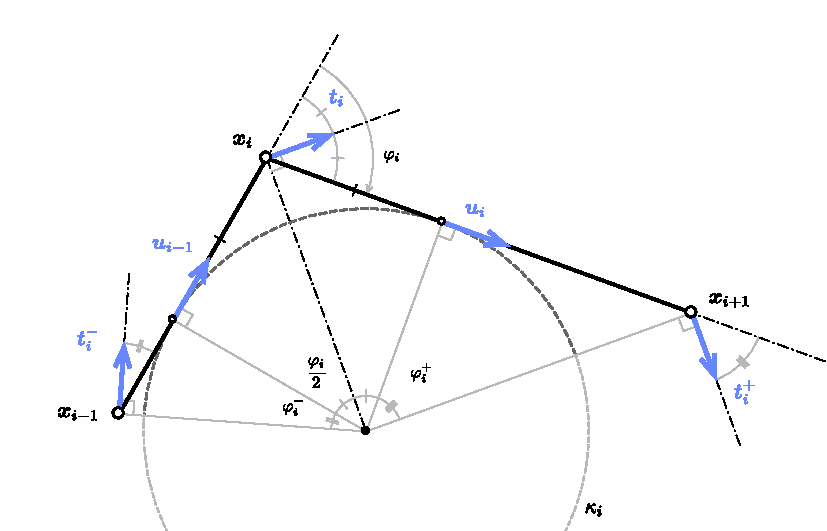
\includegraphics{kb_edge_tangent.pdf}\label{fig:kb_edge_tangent_a}}\\
	\subfloat[][start]{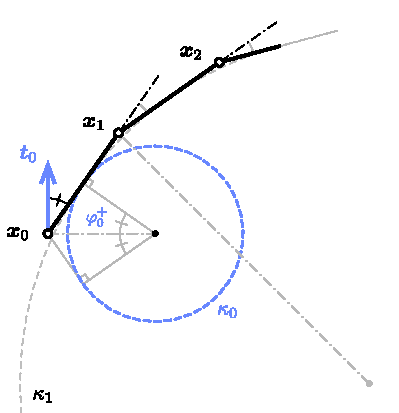
\includegraphics{kb_edge_start.pdf}\label{fig:kb_edge_tangent_b}}\hspace{5mm}
	\subfloat[][end]{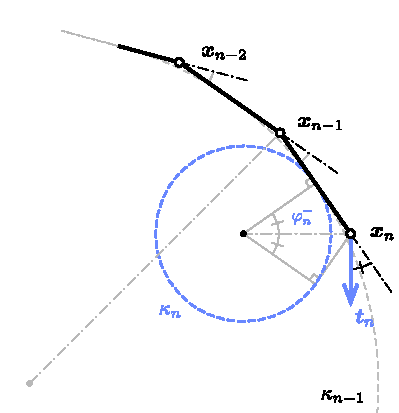
\includegraphics{kb_edge_end.pdf}\label{fig:kb_edge_tangent_c}}
	\vspace{10pt}
	\caption{Definition of the tangent vector ($\vect{t}$) and related curvature binormal vector ($\vect{\kappa b}$) at vertices (inscribed definition).}
	\label{fig:kb_edge_tangent}
\end{figure}


\subsubsection{Current portion}
Let $\vect{x}_i$ be a vertex in the current portion of $\Gamma$. The inscribed osculating circle gives a smooth approximation of $\Gamma$ in the vicinity of $\vect{x}_i$ (see \cref{fig:kb_edge_tangent_a}) ; though this approximation does not pass through the vertices. It is again possible to construct some unit tangent vectors based on this circle, but the analytic expressions are less compact than in the circumscribed case (resp. at $\vect{x}_{i-1}$, $\vect{x}_i$, $\vect{x}_{i+1}$) :
\begin{subequations}
\setlength{\jot}{6pt}
\begin{alignat}{4}
	&\vect{t}_i^- 			& \quad 	&= 	 \quad 	&& \cos(\frac{\varphi_i}{2} + \varphi_i^-) \frac{\vect{u}_{i-1} + \vect{u}_{i}}{\norm{\vect{u}_{i-1} + \vect{u}_{i}}} 
											+\sin(\frac{\varphi_i}{2} + \varphi_i^-) \frac{\vect{u}_{i-1} - \vect{u}_{i}}{\norm{\vect{u}_{i-1} - \vect{u}_{i}}}  
											&\hspace{10mm}	& \\
	&\vect{t}_i 			& 		&=	 		&&\frac{\vect{u}_{i-1} + \vect{u}_{i}}{\norm{\vect{u}_{i-1} + \vect{u}_{i}}}  		
											&				& \\
	&\vect{t}_i^+ 			& 		&= 	 		&& \cos(\frac{\varphi_i}{2} + \varphi_i^+) \frac{\vect{u}_{i-1} + \vect{u}_{i}}{\norm{\vect{u}_{i-1} + \vect{u}_{i}}} 
											-\sin(\frac{\varphi_i}{2} + \varphi_i^+) \frac{\vect{u}_{i-1} - \vect{u}_{i}}{\norm{\vect{u}_{i-1} - \vect{u}_{i}}}  
										&\hspace{10mm}	&
\end{alignat}
\end{subequations}
In this form, the expressions of $\vect{t}_i^-$ and $\vect{t}_i^+$ exhibit lots of trigonometric computations. Consequently, they will be more costly to evaluate (numerically) than the ones given for the circumscribed case that exhibit only simple addition, product and division operations.

Though these points does not generally fall into mid-edge, the tangent vector can also be identified to $\vect{u}_{i-1}$ (resp. $\vect{u}_{i}$) at point $\tilde{\vect{x}}_i^- = \vect{x}_i - \frac{1}{2}\overbar{l_i} \vect{u}_{i-1}$ (resp. $\tilde{\vect{x}}_i^+ = \vect{x}_i + \frac{1}{2}\overbar{l_i} \vect{u}_{i}$) :
\begin{subequations}
\setlength{\jot}{6pt}
\begin{alignat}{4}
	&\tilde{\vect{t}}_i^- 	& \quad	&=	\quad 		&&\vect{u}_{i-1}		
											&				& \\
	&\tilde{\vect{t}}_i^+ 	& 		&=	 			&&\vect{u}_{i}  												
											&				&
\end{alignat}
\end{subequations}
Similarly to the circumscribed case, one can remark that the curvature binormal vector at $\vect{x}_i$ can be computed in three different manners :
\begin{equation}
	\vect{\kappa b}_i = \frac{2}{\overbar{l_i}} \left( \frac{\vect{e}_{i-1} \times \vect{e}_{i}}{\norm{\vect{e}_{i-1}} \norm{\vect{e}_{i}} + \vect{e}_{i-1} \cdot \vect{e}_{i}} \right)
	=
	\left \{
	\begin{aligned}	
		&  \frac{2}{\overbar{l_i}} \left(\frac{\vect{e}_{i-1} \times  \vect{t}_{i}}{\vect{e}_{i-1} \cdot \vect{t}_{i}}  \right) 
%		= \frac{2}{\norm{\vect{e}_{i-1}}} \vect{t}_{i-1} \times  \vect{u}_{i-1}
		\\[8pt]
		&  \frac{2}{\overbar{l_i}} \left( \frac{\vect{t}_{i} \times  \vect{e}_{i} }{ \vect{t}_{i} \cdot \vect{e}_{i}} \right) 
%		= \frac{2}{\norm{\vect{e}_{i}}} \vect{u}_{i} \times  \vect{t}_{i+1} 
	\end{aligned}
	\right.
\label{eq:edge_kbs}
\end{equation}
The first expression is interpreted as the unique circle bitangent to $\vect{e}_{i-1}$ at $\tilde{\vect{x}}_i^-$ and $\vect{e}_{i}$ at $\tilde{\vect{x}}_i^+$, as explained in \cref{sec:inscribed}. Equivalently, the last two expressions in \cref{eq:edge_kbs} can be interpreted as the curvature binormal vector of the unique circle which center is on the line normal to $\vect{t}_{i}$ passing through $\vect{x}_i$, and that is tangent to $\vect{e}_{i-1}$ (resp. $\vect{e}_{i}$) at $\tilde{\vect{x}}_i^-$ (resp. $\tilde{\vect{x}}_i^+$).

\subsubsection{Discontinuity of curvature}
Let $\vect{t}_i^*$ be an arbitrary tangent vector at $\vect{x}_i$. Following \cref{eq:edge_kbs} we define the \emph{left-sided} (resp. \emph{right-sided}) discrete curvature at $\vect{x}_i$ in the inscribed case as :
\begin{subequations}
\setlength{\jot}{8pt}
\begin{alignat}{2}
	&\vect{\kappa b}_{i}^-(\vect{t}_i^*) 	&&=  \frac{2}{\overbar{l_i}} \left(\frac{\vect{e}_{i-1} \times  \vect{t}_{i}^*}{\vect{e}_{i-1} \cdot \vect{t}_{i}^*} \right) \\
	&\vect{\kappa b}_{i}^+(\vect{t}_i^*)	&&= \frac{2}{\overbar{l_i}} \left( \frac{\vect{t}_{i}^* \times  \vect{e}_{i} }{ \vect{t}_{i}^* \cdot \vect{e}_{i}} \right) 
\end{alignat}
\end{subequations}
The corresponding osculating circle will be called the \emph{left-sided} (resp. \emph{right-sided}) inscribed osculating circle. When $\vect{t}_i^* = \vect{t}_i$, the limits agree one to each other ($\vect{\kappa b}_{i}^- = \vect{\kappa b}_{i}^+ = \vect{\kappa b}_{i}$) and the osculating circles coincide. These definitions perfectly mimic the smooth case where, at a regular ($\norm{\gamma'} \neq 0$) but not biregular ($\norm{\gamma''} = 0$) point, the curvature is discontinuous while the tangent vector reminds smoothly defined.




\subsubsection{Curve endings}
The definition of the left and right sided curvatures given for a vertex in the current portion of $\Gamma$ are still valid for the end vertices $\vect{x}_{0}$ and $\vect{x}_{n}$. Provided that a unit tangent vector $\vect{t}_{0}^*$ (respectively $\vect{t}_{n}^*$) is given at $\vect{x}_{0}$ (resp. $\vect{x}_{n}$), the circumscribed osculating circle is defined as the unique circle passing through $\vect{x}_0$ and $\vect{x}_1$ (resp. $\vect{x}_{n-1}$ and $\vect{x}_n$) tangent to $\vect{t}_{0}^*$ (resp. $\vect{t}_{n}^*$) ; see \cref{fig:kb_edge_tangent_b} and \cref{fig:kb_edge_tangent_c}. It leads to the following curvature binormal vectors :
\begin{subequations}
\setlength{\jot}{8pt}
\begin{alignat}{2}
	&\vect{\kappa b}_0 =\vect{\kappa b}_{0}^+(\vect{t}_0^*)	&&=  \frac{2}{\norm{\vect{e}_{0}}} \left( \frac{\vect{t}_{0}^* \times  \vect{e}_{0} }{ \vect{t}_{0}^* \cdot \vect{e}_{0}} \right) \\
	&\vect{\kappa b}_n =\vect{\kappa b}_{n}^-(\vect{t}_n^*) 	&&=  \frac{2}{\norm{\vect{e}_{n-1}}} \left(\frac{\vect{e}_{n-1} \times  \vect{t}_{n}^*}{\vect{e}_{n-1} \cdot \vect{t}_{n}^*} \right) 
\end{alignat}
\end{subequations}
Note that, contrary to the current portion, curvatures at endings are subjected to the definition of a unit tangent vector. This reflects the usual indetermination of boundary conditions. For a given beam whether the end is clamped, the tangent vector is known and one will seek the reacting moment due to the support ; whether the end is pinned, the reacting moment is null (so is the curvature) and one will seek the cross section orientation.

% DISCRETE FRAMES
% =================
\section{Discrete parallel transport}

Discrete parallel transport can be computed by anaolgy to the smooth case as the rotation minimizing rotation around t :
This methods is unstable when t1 an t2 gets almost colinear.

Note that while these definitions of parallel transport are illustrated to transport vectors in space from one location $\{\vect{x},\vect{t}\}(s)$ to another $\{\vect{x},\vect{t}\}(s + ds)$, it is identically transposed to parallel transport in time from one location $\{\vect{x},\vect{t}\}(t)$ to another $\{\vect{x},\vect{t}\}(t+dt)$ as suggested in \cite{Bergou2010}.

\subsection{The rotation method}

The rotation method is given in \cite{Bloomenthal1990}. First, the frame at $\vect{x}_i$ is simply translated at vertex $\vect{x}_{i+1}$. Then, the translated frame is rotated so that $\vect{t}_i$ aligns with $\vect{t}_{i+1}$. The rotation axis is chosen to be $\vect{b} = \vect{t}_i \times \vect{t}_{i+1}$ and the angle of rotation is denoted $\alpha$ (see \cref{fig:pt_rotation}). This is analogous as the smooth case.

\begin{figure}[!p]
	\captionsetup[subfloat]{captionskip=10pt}
	\centering
	\subfloat[][rotation method]{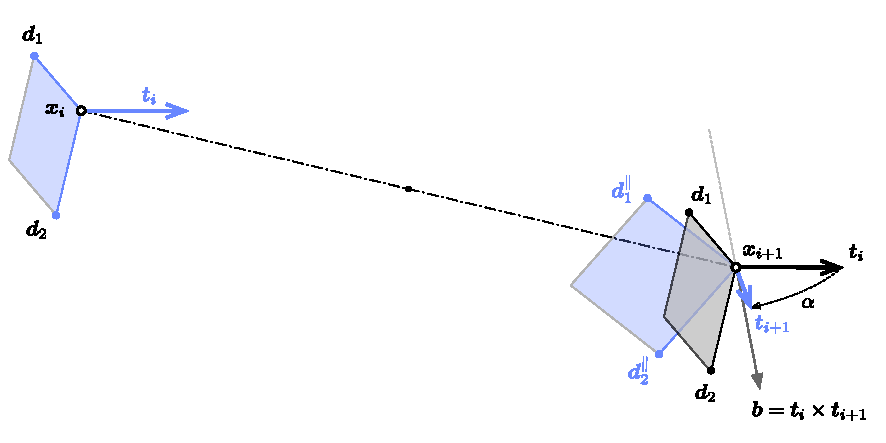
\includegraphics{pt_rotation.pdf}\label{fig:pt_rotation}}\\
	\subfloat[][double reflection method]{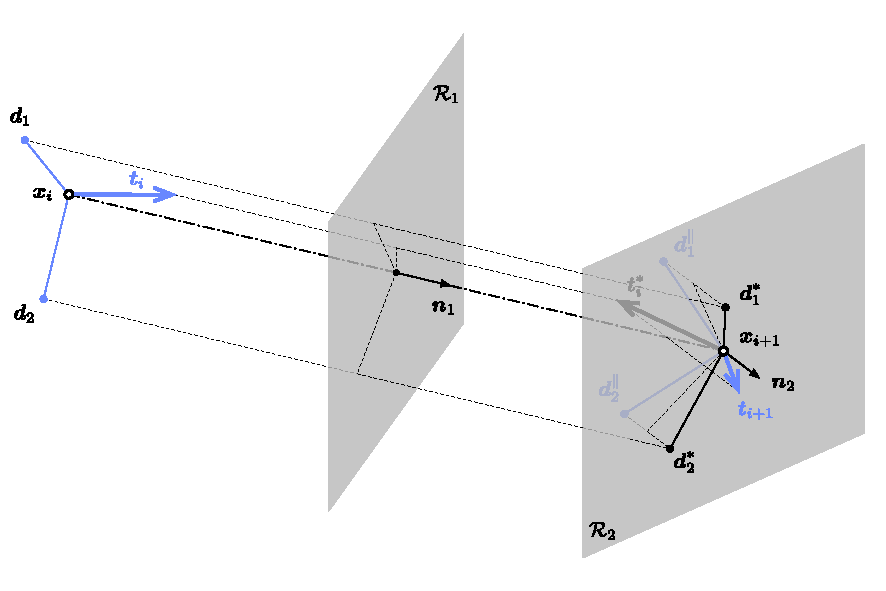
\includegraphics{pt_reflection.pdf}\label{fig:pt_reflection}}
	\vspace{10pt}
	\caption{Parallel transport of vectors from $\{\vect{x}_i,\vect{t}_i\}$ to $\{\vect{x}_{i+1},\vect{t}_{i+1}\}$.}
	\label{fig:pt}
\end{figure}

%\begin{figure}[!tb]
%	\centering
%	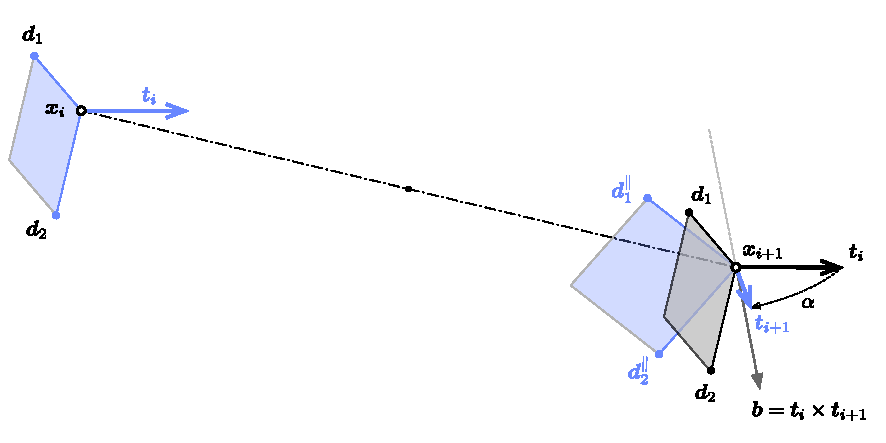
\includegraphics[]{pt_rotation.pdf}
%	\caption{Discrete parallel transport (rotation method).}
%	\label{fig:pt_rotation}
%	
%	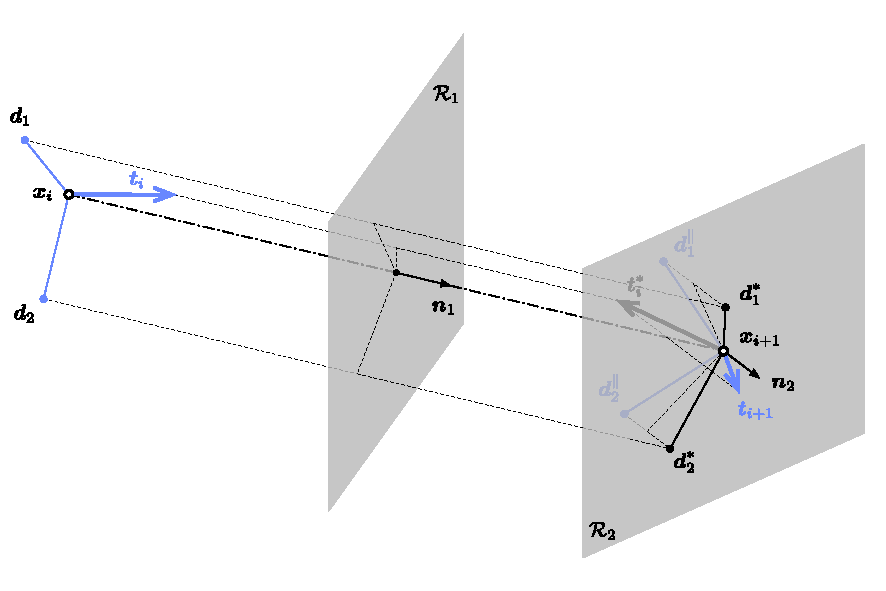
\includegraphics[]{pt_reflection.pdf}
%	\caption{Discrete parallel transport (double reflection method).}
%	\label{fig:pt_reflection}
%\end{figure}

\subsection{The double reflexion method}
%\begin{figure}[t]
%	\centering
%	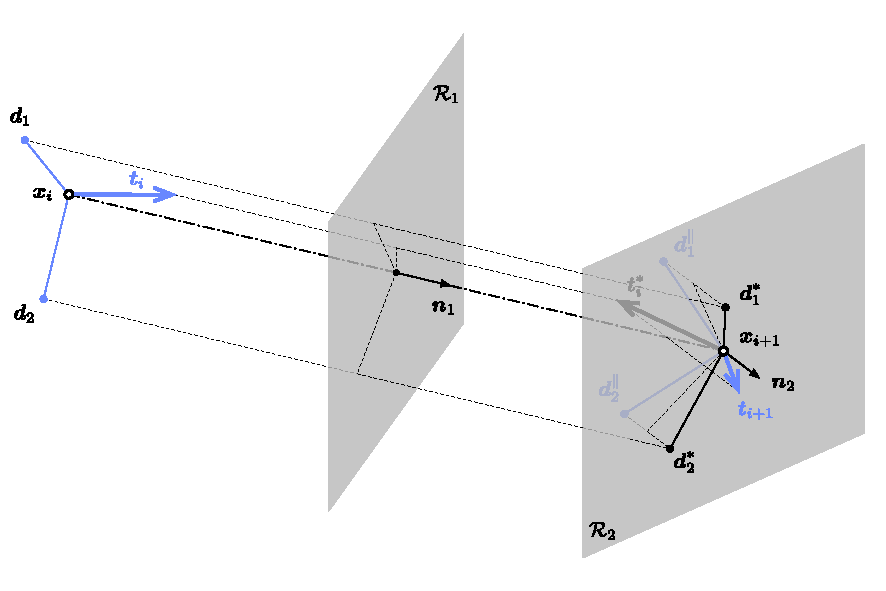
\includegraphics[]{pt_reflection.pdf}
%	\caption{Discrete parallel transport (double reflection method).}
%	\label{fig:pt_reflection}
%\end{figure}

The double reflection method is given by \cite{Wang2008}. It is supposed to be of order $o(h^4)$ whereas the rotation method is only $o(h^2)$, where $h = \sup_{i\in \llbracket 0,1 \rrbracket} \norm{\vect{e}_i}$ is the sharpness of the discretization. Though their computation cost is quite similar, the double reflection method is not subjected to instability when $\vect{t}_i$ and $\vect{t}_{i+1}$ tend to be collinear, which is an obvious advantage.

We denote $\mathcal{R}_{\vect{x}}^{\vect{n}}$ the reflection across the plane passing through the point $\vect{x}$ and normal to the vector $\vect{n}$ of unit length ($\norm{\vect{n}}=1$). Thus, $\vect{v}$ is maped through $\mathcal{R}$ into $\vect{v}^* = \vect{v} - 2(\vect{v}\cdot\vect{n})\vect{n}$.

Let $\mathcal{R}_{1} = \mathcal{R}_{\vect{x}_{i+1/2}}^{\vect{n}_{1}}$ be the reflection across the bisecting plane of $\vect{e}_i$ ($\vect{n}_{1} = \vect{u}_i$).
Let $\vect{t}_i^* = \mathcal{R}_{1}(\vect{t}_i)$ be the image of $\vect{t}_i$ by $\mathcal{R}_{1}$.
Let $\mathcal{R}_{2} = \mathcal{R}_{\vect{x}_{i+1}}^{\vect{n}_{2}}$ be the reflection across the bisecting plane of the points $\vect{x}_{i+1} + \vect{t}_i^*$ and $\vect{x}_{i+1} + \vect{t}_{i+1}$. 
Thus, $\vect{n}_{2} = \frac{ \vect{t}_{i+1} - \vect{t}_i^*}{\norm{\vect{t}_{i+1} - \vect{t}_i^*}}$ (see \cref{fig:pt_reflection}).

The parallel transport is defined as the \emph{double reflection} through $\mathcal{R}_{1}$ and $\mathcal{R}_{2}$ :
\begin{equation}
	\mathcal{P}_{\{\vect{x}_{i}, \, \vect{t}_{i}\}}^{\{\vect{x}_{i+1}, \,\vect{t}_{i+1}\}} = \mathcal{P}_i^{i+1} = \mathcal{R}_{2} \circ \mathcal{R}_{1}
\end{equation}
Let $\mathcal{F}_i = \{ \vect{t}_i, \vect{d}_1, \vect{d}_2 \}$ be an orthonormal frame at $\vect{x}_i$. 
Let $\mathcal{F}_i^* = \mathcal{R}_{1}(\mathcal{F}_i) = \{ \vect{t}_i^*, \vect{d}_{1}^*, \vect{d}_{2}^* \}$ be the image of $\mathcal{F}_i$ by $\mathcal{R}_{1}$. 
Then : 
\begin{subequations}
\begin{alignat}{3}
	&\vect{t}_i^* 	&&= \vect{t}_i - 2 (\vect{t}_i \cdot \vect{n}_1) \vect{n}_1 \\
	&\vect{d}_1^* 	&&= \vect{d}_1 - 2 (\vect{d}_1 \cdot \vect{n}_1) \vect{n}_1 \\
	&\vect{d}_2^* 	&& = \vect{d}_1^* \times \vect{t}_i^*
\end{alignat}
\end{subequations}
Let $\mathcal{F}_i^{\parallel} = \mathcal{R}_{2} (\mathcal{F}_i^*) = \{ \vect{t}_{i+1}, \vect{d}_1^{\parallel}, \vect{d}_2^{\parallel} \}$ be the image of $\mathcal{F}_i^*$ by $\mathcal{R}_{2}$. Then the parallel transported vectors are given by :
\begin{subequations}
\begin{alignat}{3}
	&\vect{d}_1^{\parallel} 	&&= \vect{d}_1^* - 2 (\vect{d}_1^* \cdot \vect{n}_2) \vect{n}_2 \\
	&\vect{d}_2^{\parallel}	&& = \vect{t}_{i+1} \times \vect{d}_1^{\parallel}
\end{alignat}
\end{subequations}
The double reflection is equivalent to a rotation around the line $\mathcal{D}$ defined as the intersection of the two reflection planes, of direction $\vect{b} = \vect{n}_{1} \times \vect{n}_{2}$, by an angle $\alpha = 2\angle(\vect{n}_1, \vect{n}_2) = 2\arcsin (\norm{\vect{b}})$. 

\note{Ici il faudrait calculer les coordonnées du centre de rotaion. Idem pour la méthode par rotation (translation + rotation = rotation ??) => trouver l'axe de rotation, l'angle et le centre la rotation équivalente. Comparer les méthodes.}

Remark that for both the circumscribed (see \cref{fig:kb_vertex_tangent_a}) and inscribed (see \cref{fig:kb_edge_tangent_a}) osculating circles :
\begin{subequations}
\begin{alignat}{3}
	&\vect{t}_i 	&&= \mathcal{R}_{\vect{x}_{i-1/2}}^{\vect{u}_{i-1}} \circ \mathcal{R}_{\vect{x}_{i}}^{\vect{t}_{i}}  (\vect{t}_i^-) \\
	&\vect{t}_i 	&&= \mathcal{R}_{\vect{x}_{i}}^{\vect{t}_{i}} \circ \mathcal{R}_{\vect{x}_{i+1/2}}^{\vect{u}_{i}}  (\vect{t}_i^+)
\end{alignat}
\end{subequations}

% CONCLUSION
% =================
\section{Conclusion}

Apres un rappel sur les courbes continues de l'espace, nous avons introduit, pour le cas continu, les notions de courbure, torsion géométrique, interinsèque à la courbe.
Puis nous avons introduit les repères mobiles : adapté, de Frenet, de Bishop.

Nous avons fait le passage en discret et ca augmente en complexité. EN particulier, nous avons vu que la definition de la courbure n'est pas univoque. Nous avons identifé 2 approches, que nous avons comparé. Bien que la seconde est le comportement désiré pour pénaliser les courbures importantes, l'autre présente bcp d'avantages. Localité parfaite, interpolation par un arc, compatibilité des courbures droite/gauche et 3 points. Extension de la définiiton aux extrémitées. Meilleur représentativité" de l'énergie pour une discretization régulière sur des cas classiques.

Nous avons ensuite regardé la question de la definfition du vecteur tangent pour ces 2 définitions. Et sa corrélation avec la courbure. 

En fin, nous avons exposé 2 méthodes pour le calcul du transport parallel sur une courbe discrete : la rotation et la double reflection, qui ne presente pas d'iunstabilité lorsque la courbure tend à s'annuler. (donc ti ti+1 colineaires).

%
%$\vect{d}_{1,i}^{' }$
%
%${\vect{d}_{i}^{1}}^{'}$
%
%$\vect{d}_{i}^{1,*}$
%
%$\vect{d}_{1,i}^{*}$
%
%$\vect{d}_{1,i}^{\perp}$
%
%$\vect{d}_{1,i}^{\parallel}$
%
%$\vect{d}_{1,i}^{\para}$
%
\cite{Hanson95,Wang2008}


%\begin{figure}[p]
%\begin{leftfullpage}
%	\captionsetup[subfloat]{captionskip=20pt}
%	\centering
%	\vspace{-5mm}
%	\subfloat[][current portion]{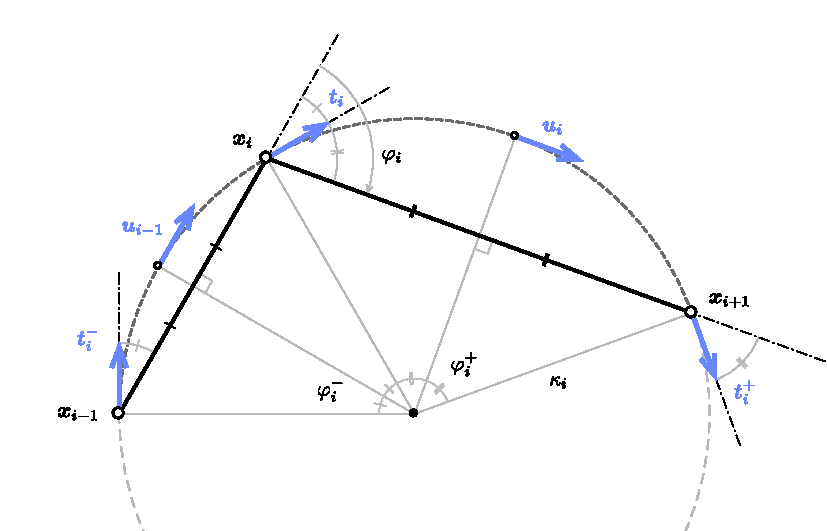
\includegraphics{kb_vertex_tangent.pdf}\label{fig:kb_vertex_tangent_a}}\\
%	\subfloat[][start]{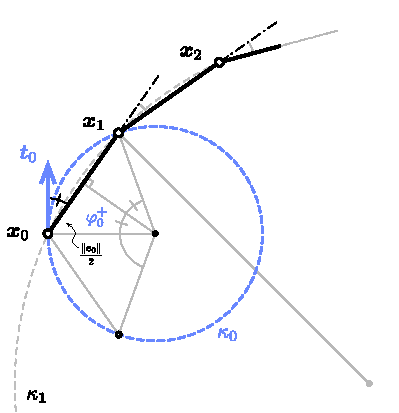
\includegraphics{kb_vertex_start.pdf}\label{fig:kb_vertex_tangent_b}}\hspace{5mm}
%	\subfloat[][end]{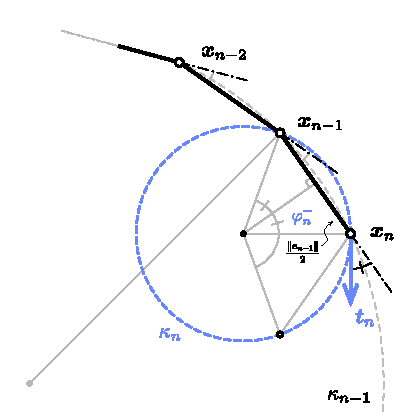
\includegraphics{kb_vertex_end.pdf}\label{fig:kb_vertex_tangent_c}}
%	\vspace{8pt}
%	\caption{Definition of the tangent vector ($\vect{t}$) and related curvature binormal vector ($\vect{\kappa b}$) at vertices (circumscribed definition).}
%	\label{fig:kb_vertex_tangent}
%\end{leftfullpage}
%\end{figure}
%\begin{figure}[p]
%\begin{fullpage}
%	\captionsetup[subfloat]{captionskip=10pt}
%	\centering
%	\vspace{-5mm}
%	\subfloat[][current portion]{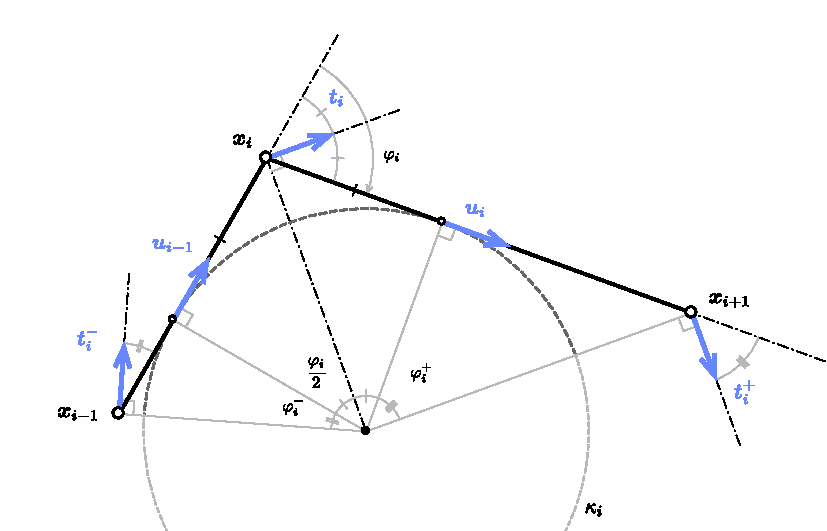
\includegraphics{kb_edge_tangent.pdf}\label{fig:kb_edge_tangent_a}}\\
%	\subfloat[][start]{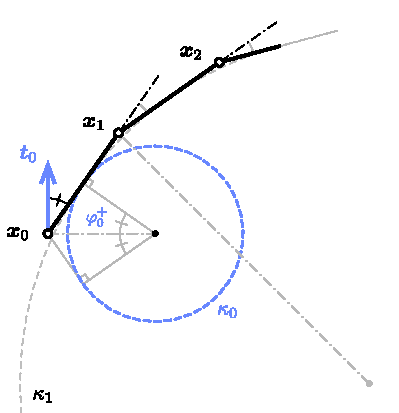
\includegraphics{kb_edge_start.pdf}\label{fig:kb_edge_tangent_b}}\hspace{5mm}
%	\subfloat[][end]{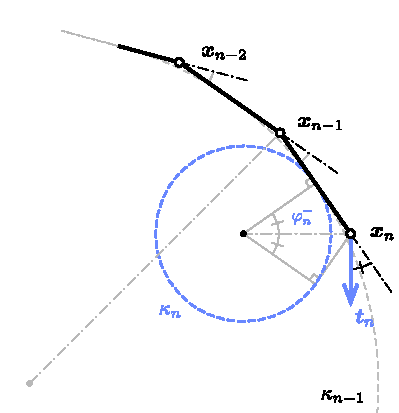
\includegraphics{kb_edge_end.pdf}\label{fig:kb_edge_tangent_c}}
%	\vspace{8pt}
%	\caption{Definition of the tangent vector ($\vect{t}$) and related curvature binormal vector ($\vect{\kappa b}$) at vertices (inscribed definition).}
%	\label{fig:kb_edge_tangent}
%\end{fullpage}
%\end{figure}

\bibliographystyle{alpha}
\bibliography{../library}
